\documentclass{article}

% 导入宏包
\usepackage{fancyhdr}
\usepackage{ctex}
\usepackage{listings}
\usepackage{graphicx}
\usepackage[a4paper, body={18cm,22cm}]{geometry}
\usepackage{amsmath,amssymb,amstext,wasysym,enumerate,graphicx}
\usepackage{float,abstract,booktabs,indentfirst,amsmath}
\usepackage{array}
\usepackage{multirow}
\usepackage{url}
\usepackage{diagbox}
\usepackage{enumitem}
\usepackage{xcolor}
\usepackage{makecell}
\usepackage{tikz}
\usepackage{tcolorbox}
\usetikzlibrary{positioning, arrows.meta}

% 设置段落
\renewcommand\arraystretch{1.4}
\setlength{\parindent}{2em}
\setCJKmonofont{黑体}

% 设置高亮文字
\newtcbox{\mybox}[1][red]
{on line, arc = 0pt, outer arc = 0pt,
	colback = #1!10!white, colframe = #1!50!black,
	boxsep = 0pt, left = 1pt, right = 1pt, top = 2pt, bottom = 2pt,
	boxrule = 0pt, bottomrule = 1pt, toprule = 1pt}

% 配置代码显示
\lstset{
	xleftmargin = 3em,
	xrightmargin = 3em,
	aboveskip = 1em,
	backgroundcolor = \color{white},
	basicstyle = \small\ttfamily,
	rulesepcolor = \color{gray},
	breaklines = true,
	numbers = left,
	numberstyle = \small,
	numbersep = -14pt,
	keywordstyle = \color{purple}\bfseries,
	commentstyle = \color{green!60!black}, % 修改注释颜色
	stringstyle = \color{red!60!green!90!blue!90},
	morekeywords = {ASSERT, int64_t, uint32_t},
	moreemph = {ASSERT, NULL},
	emphstyle = \color{red}\bfseries,
	moreemph = [2]{int64\_t, uint32\_t, tid\_t, uint8\_t, int16\_t, uint16\_t, int32\_t, size\_t, bool},
	emphstyle = [2]\color{purple}\bfseries,
	frame = shadowbox,
	showspaces = false,
	columns = fixed
	morecomment = [l][\color{green!60!black}]{+}, % 设置以+开头的代码行为绿色
}

%--------------------页眉--------------------%

\pagestyle{fancy}
\fancyhead[L]{}
\fancyhead[R]{}
\fancyhead[C]{华东师范大学软件工程学院实验报告}
\fancyfoot[C]{-\thepage-}
\renewcommand{\headrulewidth}{1.5pt}

%--------------------标题--------------------%

\begin{document}
	\begin{center}
		{\Large{\textbf{\heiti 华东师范大学软件工程学院实验报告}}}
		\begin{table}[htb]
			\flushleft
			\begin{tabular}{p{0.4\linewidth}p{0.27\linewidth}p{0.28\linewidth}}\\
				\textbf{实验课程}:计算机网络实践  & \textbf{年级}:2023级  & \textbf{实验成绩}:  \\
				\textbf{实验名称}:TCP  & \textbf{姓名}:顾翌炜  &                     \\
				\textbf{实验编号}:06  & \textbf{学号}:10235101527 & \textbf{实验日期}:2024/12/27  \\
				\textbf{指导教师}:王廷  & \textbf{组号}:01     & \textbf{实验时间}:2024/12/27  \\ 
			\end{tabular}
		\end{table}
	\end{center}
	\rule{\textwidth}{2pt}
	
	%--------------------正文--------------------%
	\section{实验目的}
	
	\begin{enumerate}[noitemsep, label={{\arabic*})}]
		\item 学会通过 \texttt{Wireshark}获取 \texttt{TCP}消息
		\item 掌握 \texttt{TCP}数据包结构
		\item 掌握 \texttt{TCP}数据包各字段的含义
		\item 掌握 \texttt{TCP}连接建立和释放的步骤
		\item 掌握 \texttt{TCP}数据传输阶段的过程
	\end{enumerate}
	
	\section{实验内容与实验步骤}
	
	\subsection{实验内容}
	
	\begin{enumerate}[noitemsep, label={{\arabic*})}]
		\item 捕获并检查获取到的包
		\item 分析TCP结构
		\item 分析TCP连接建立和释放的过程
		\item 分析TCP数据传输的过程
	\end{enumerate}\textbf{}
	
	\subsection{实验步骤}
	
	\begin{enumerate}[noitemsep, label={{\arabic*})}]
		\item 输入以下指令,用wget确认链接有效。
		
		\begin{lstlisting}[language=bash]
        C:\User\GHOST> wget http://img.zcool.cn/community/01dcd059117b12a801216a3e9c4fd5.jpg
		\end{lstlisting}
		
		\item 启动\texttt{Wireshark},在菜单栏的捕获 \( \to \) 选项中进行设置,选择已连接的以太网,设置捕获过滤器为\texttt{tcp and host img.zcool.cn}。我们主要观察客户端与服务器之间的\texttt{tcp}流。
		\item 捕获开始后,重复第一步,重新发送请求。
		\item 当\texttt{wget}命令结束后,停止\texttt{Wireshark}捕获。
	\end{enumerate}\textbf{}
	
	\section{实验环境}
	
	\begin{itemize}[noitemsep]
		\item 操作系统:\texttt{Windows 11 家庭中文版 23H2 22631.4460}
		\item 网络适配器:\texttt{Killer(R)Wi-Fi 6E AX1675i 160MHz Wireless Network Adapter(211NGW)}
		\item \texttt{Wireshark}:\texttt{Version 4.4.1}
		\item \texttt{wget}:\texttt{GNU Wget 1.21.4 built on mingw32}
	\end{itemize}
	
	\section{实验过程与分析}
	
	\subsection{捕获 \texttt{TCP} 报文}
	
	首先,我们使用 \texttt{wget} 确认链接有效。
	
	\begin{figure}[H]
		\centering
		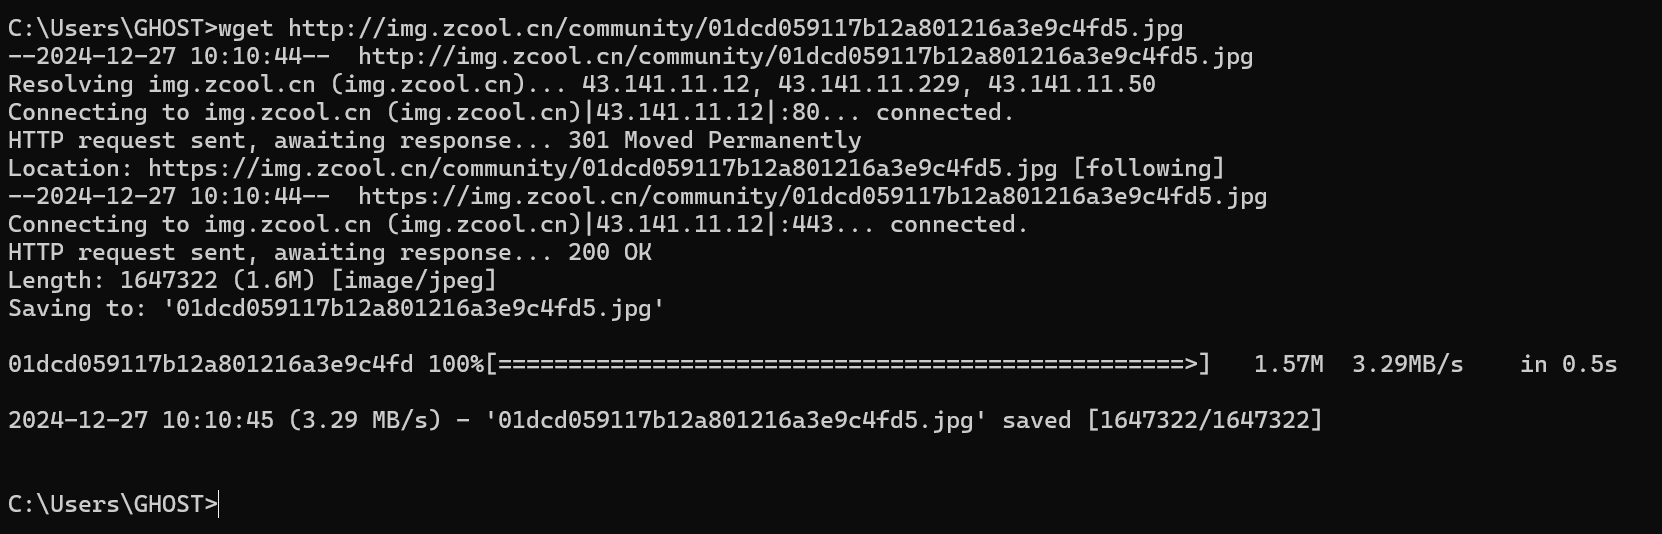
\includegraphics[width=11cm]{images/1.使用wget确认链接有效.png}
		\caption{使用wget确认链接有效}
	\end{figure}
	
	然后,我们启动\texttt{Wireshark},在菜单栏的捕获 \( \to \) 选项中进行设置,选择已连接的以太网,设置捕获过滤器为\texttt{tcp and host img.zcool.cn}。
	
	\begin{figure}[H]
		\centering
		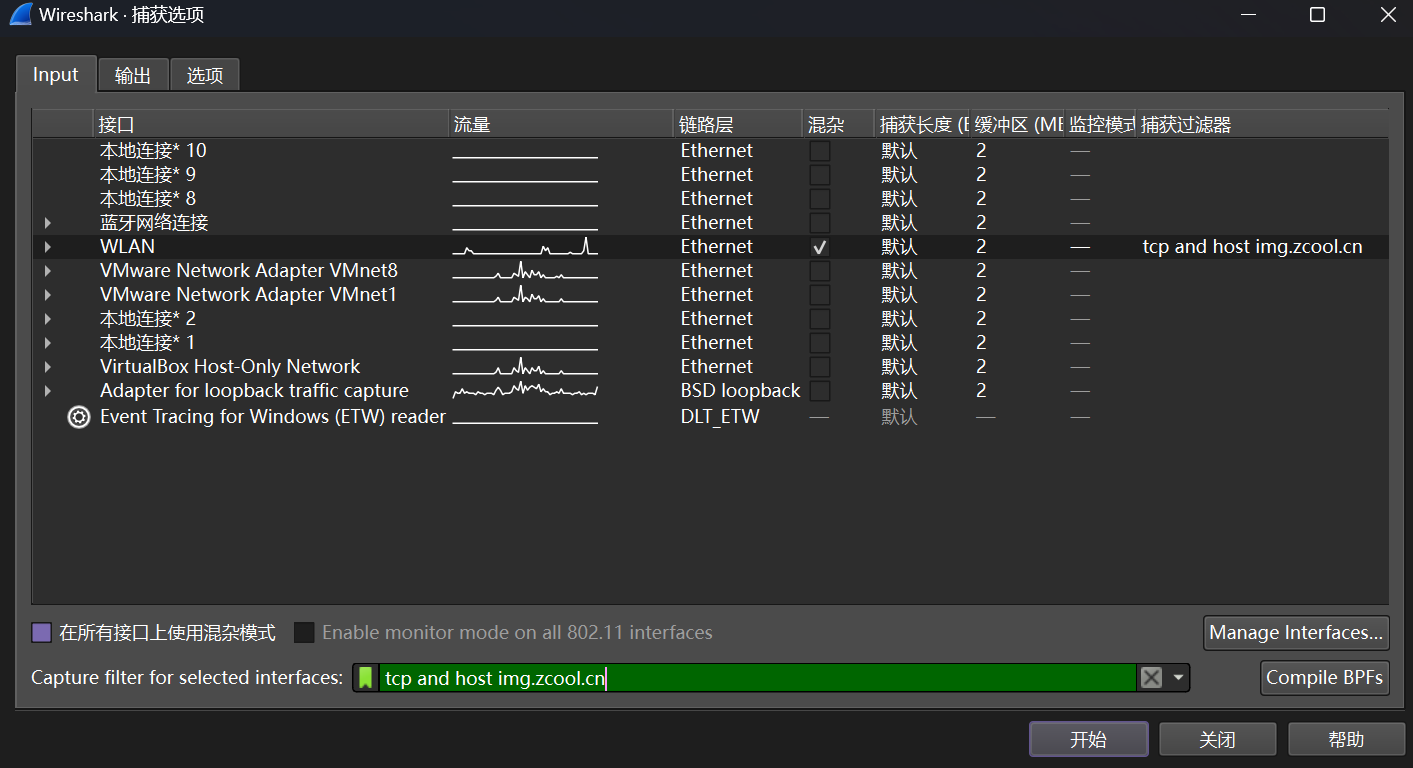
\includegraphics[width=11cm]{images/2.设置捕获.png}
		\caption{设置捕获}
	\end{figure}
	
	捕获开始后,重复第一步,重新发送请求。
	
	当\texttt{wget}命令结束后,停止\texttt{Wireshark}捕获。
	
	捕获结果如下:
	
	\begin{figure}[H]
		\centering
		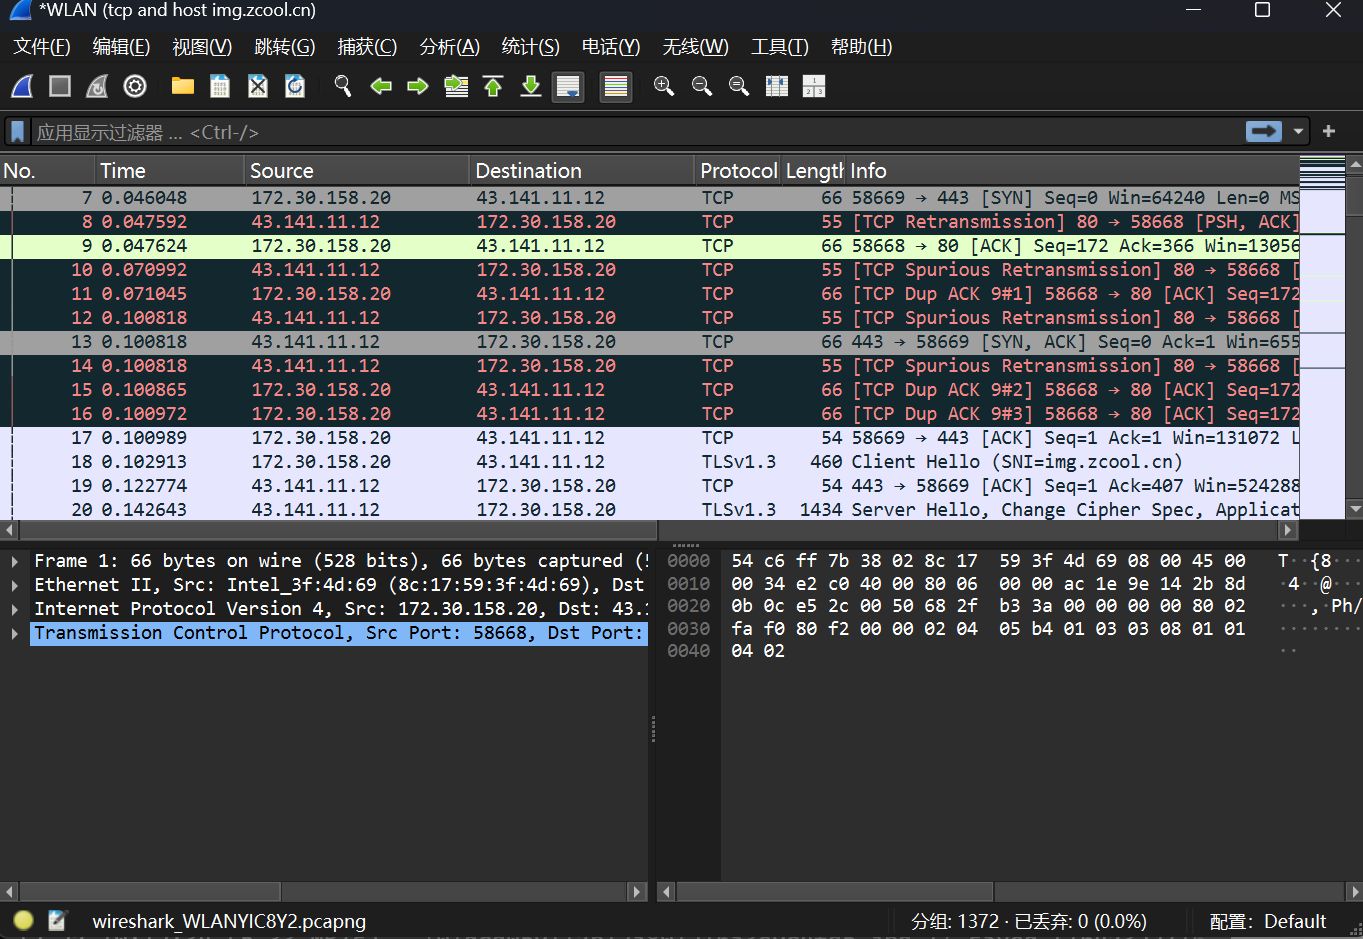
\includegraphics[width=11cm]{images/3.捕获结果.png}
		\caption{捕获结果}
	\end{figure}
	
	\subsection{分析 \texttt{TCP} 报文}
	
	选择一个\texttt{TCP}数据包,如下所示:
	
	\begin{figure}[H]
		\centering
		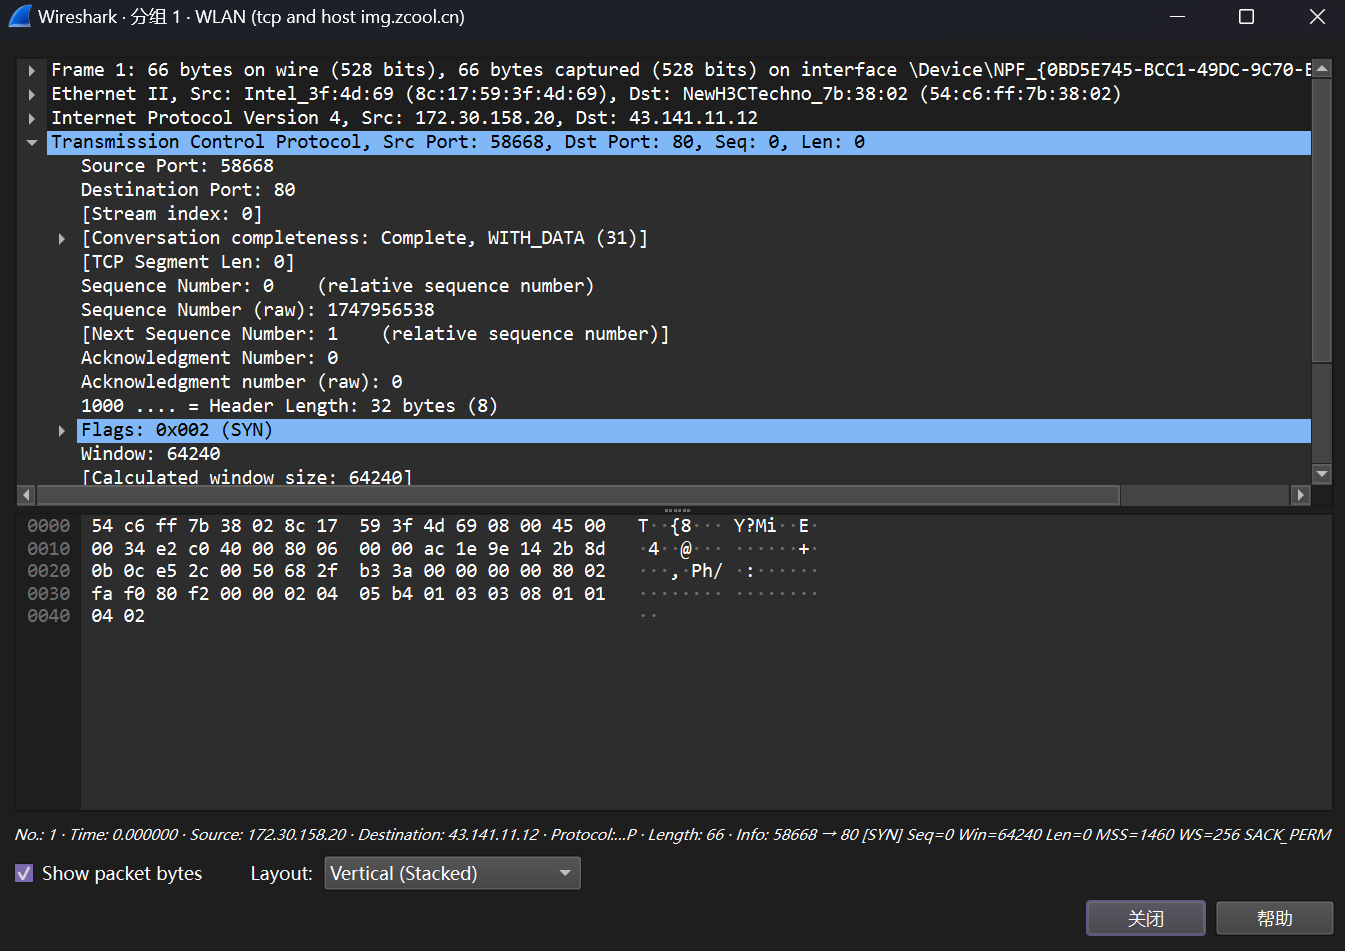
\includegraphics[width=0.6\textwidth]{images/4.TCP 数据包.png}
		\caption{TCP 数据包}
	\end{figure}
	
	具体来看每一个部分的信息:
	
	\begin{figure}[H]
		\centering
		\begin{minipage}[b]{0.45\textwidth}
			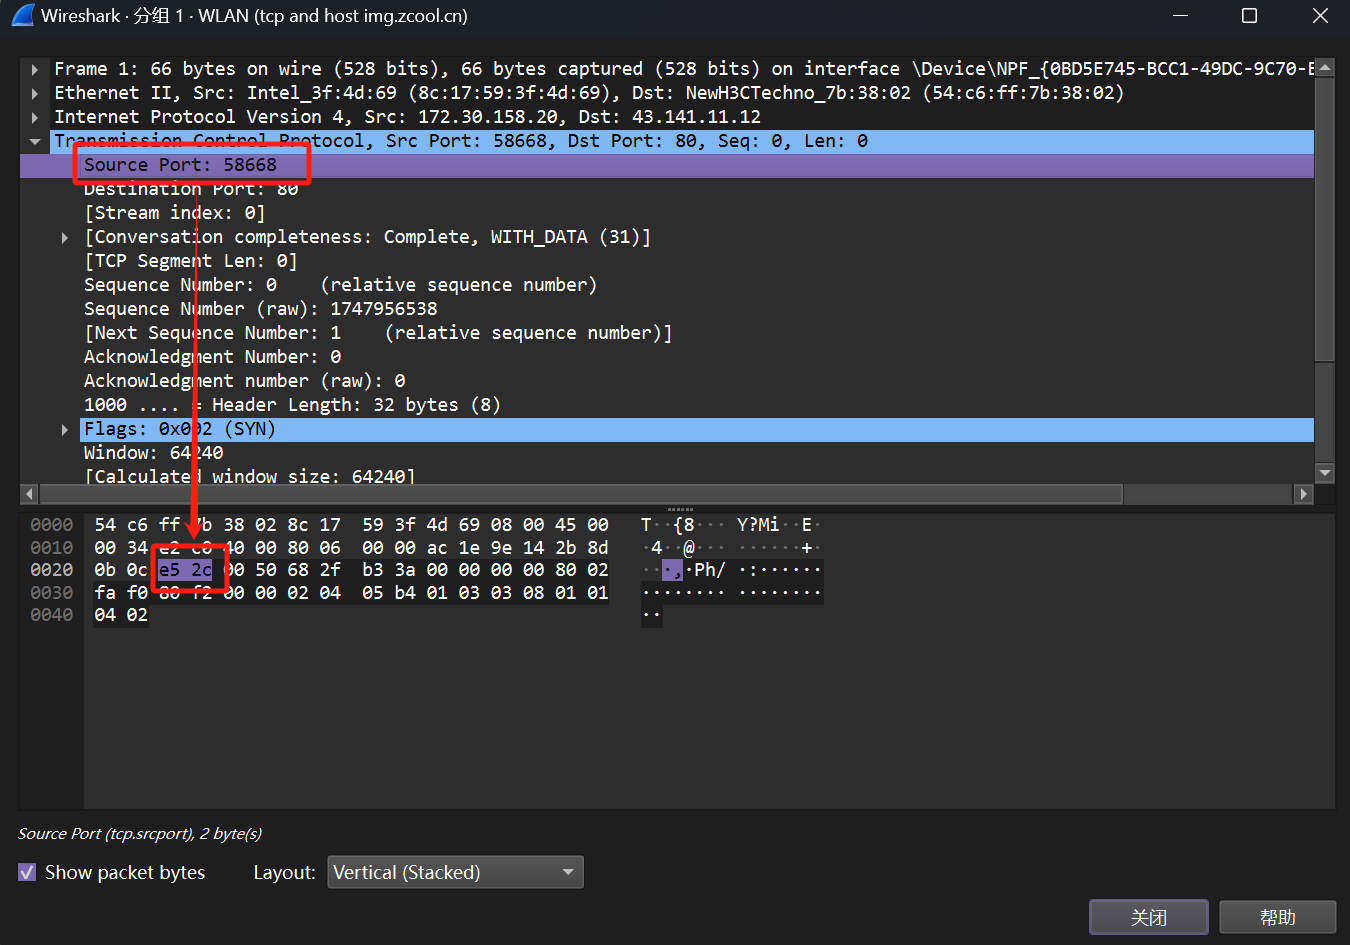
\includegraphics[width=\textwidth]{images/5.Source Port.png}
			\caption{Source Port}
		\end{minipage}
		\hfill
		\begin{minipage}[b]{0.45\textwidth}
			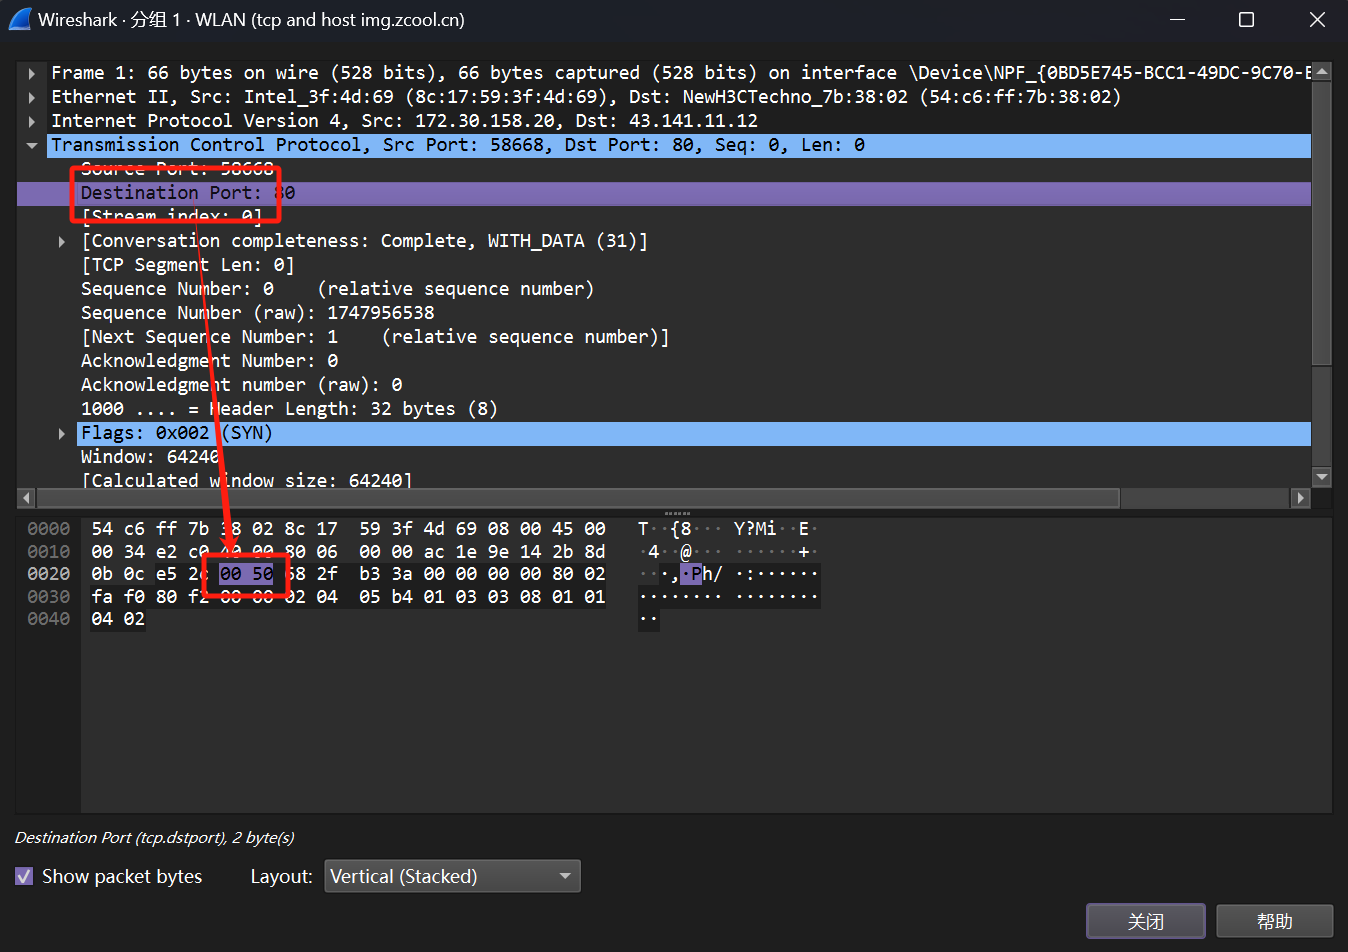
\includegraphics[width=\textwidth]{images/6.Destination Port.png}
			\caption{Destination Port}
		\end{minipage}
	\end{figure}
	
	\begin{figure}[H]
		\centering
		\begin{minipage}[b]{0.45\textwidth}
			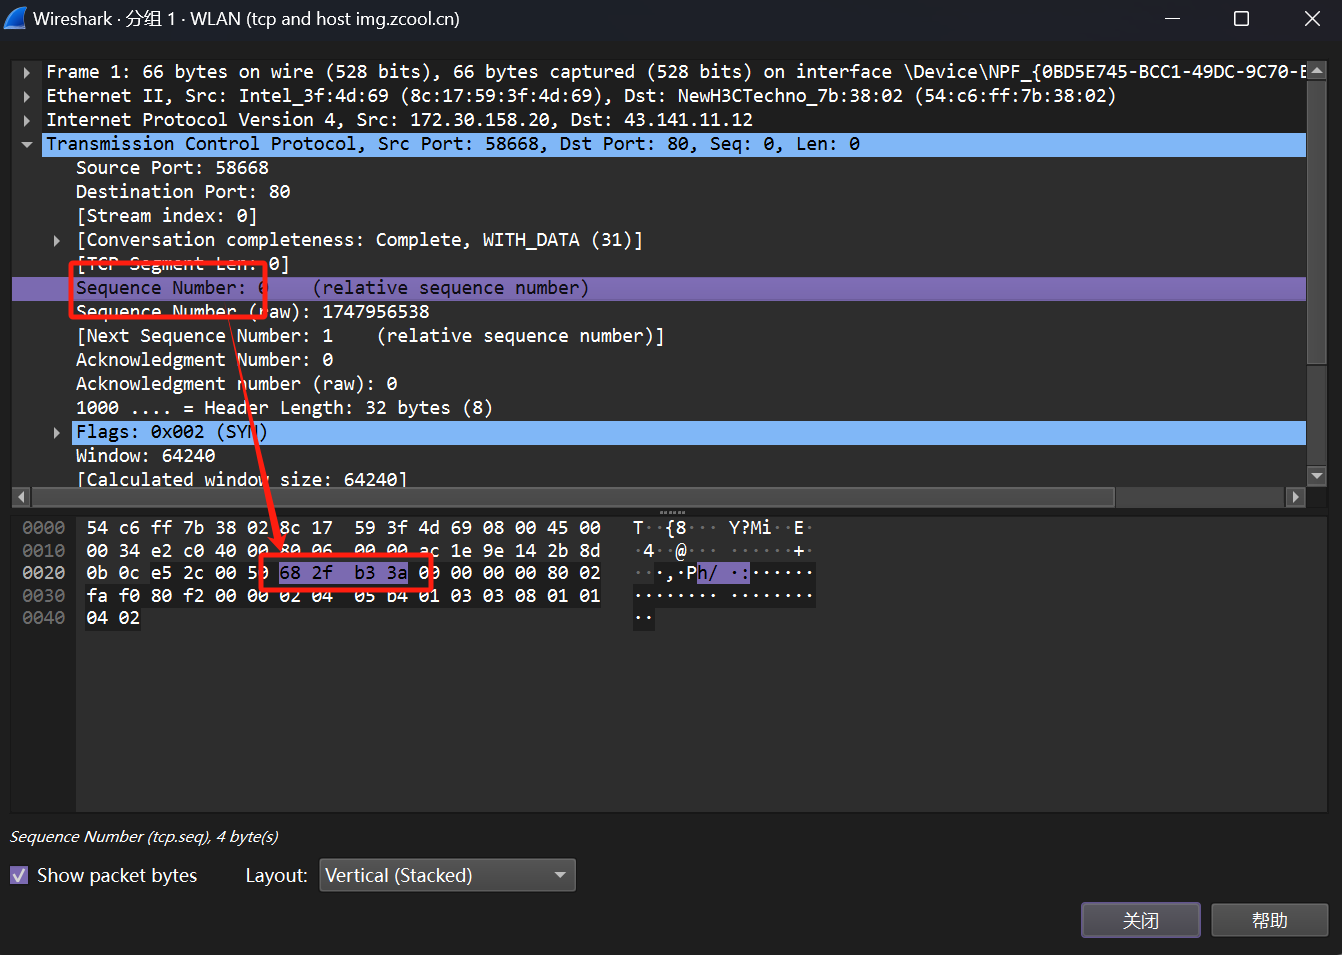
\includegraphics[width=\textwidth]{images/7.Sequence Number.png}
			\caption{Sequence Number}
		\end{minipage}
		\hfill
		\begin{minipage}[b]{0.45\textwidth}
			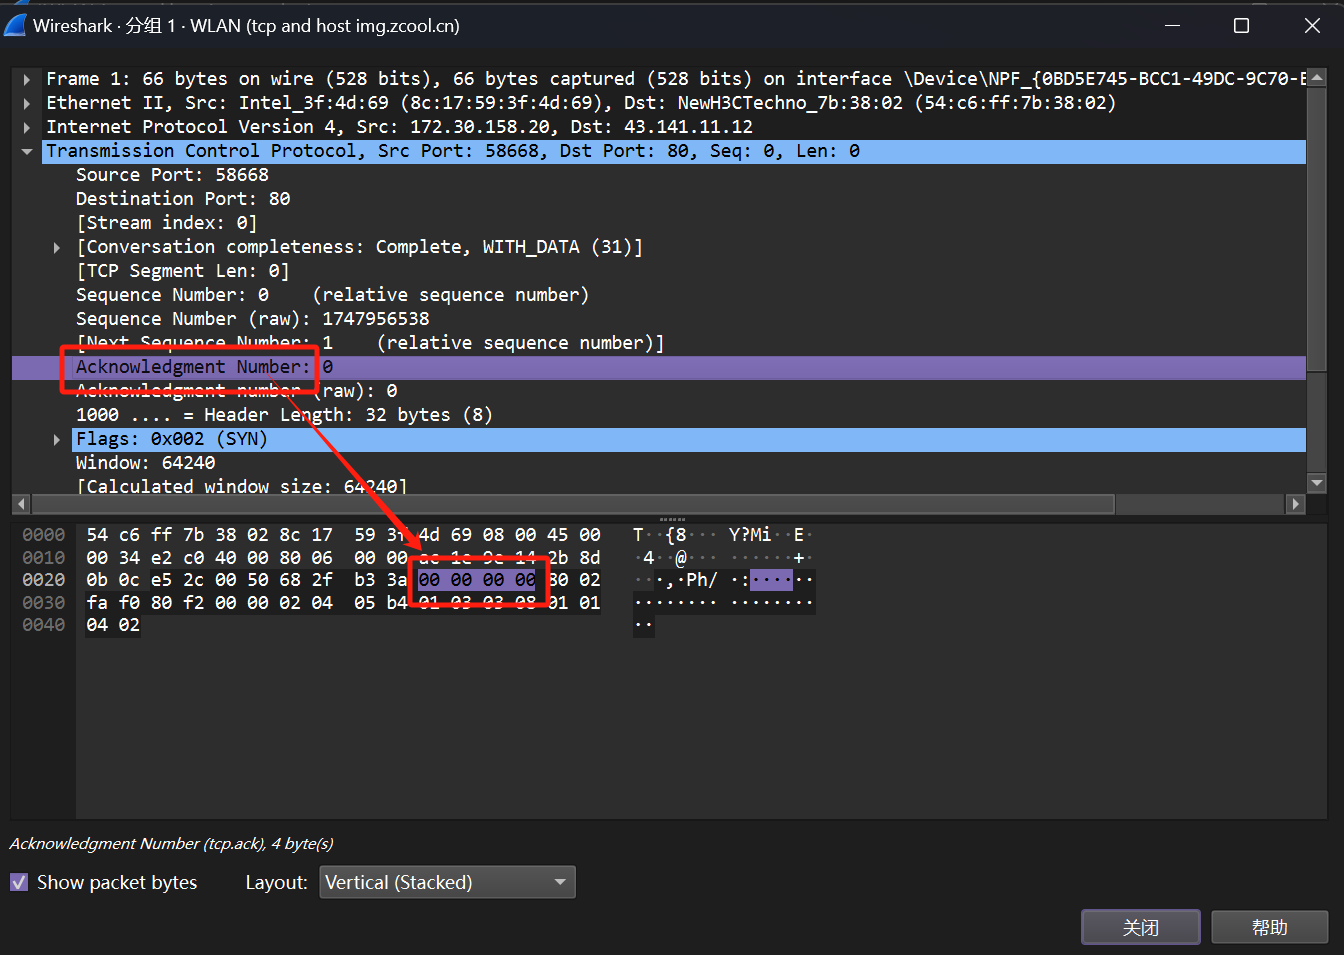
\includegraphics[width=\textwidth]{images/8.Acknowledge Number.png}
			\caption{Acknowledge Number}
		\end{minipage}
	\end{figure}
	
	\begin{figure}[H]
		\centering
		\begin{minipage}[b]{0.45\textwidth}
			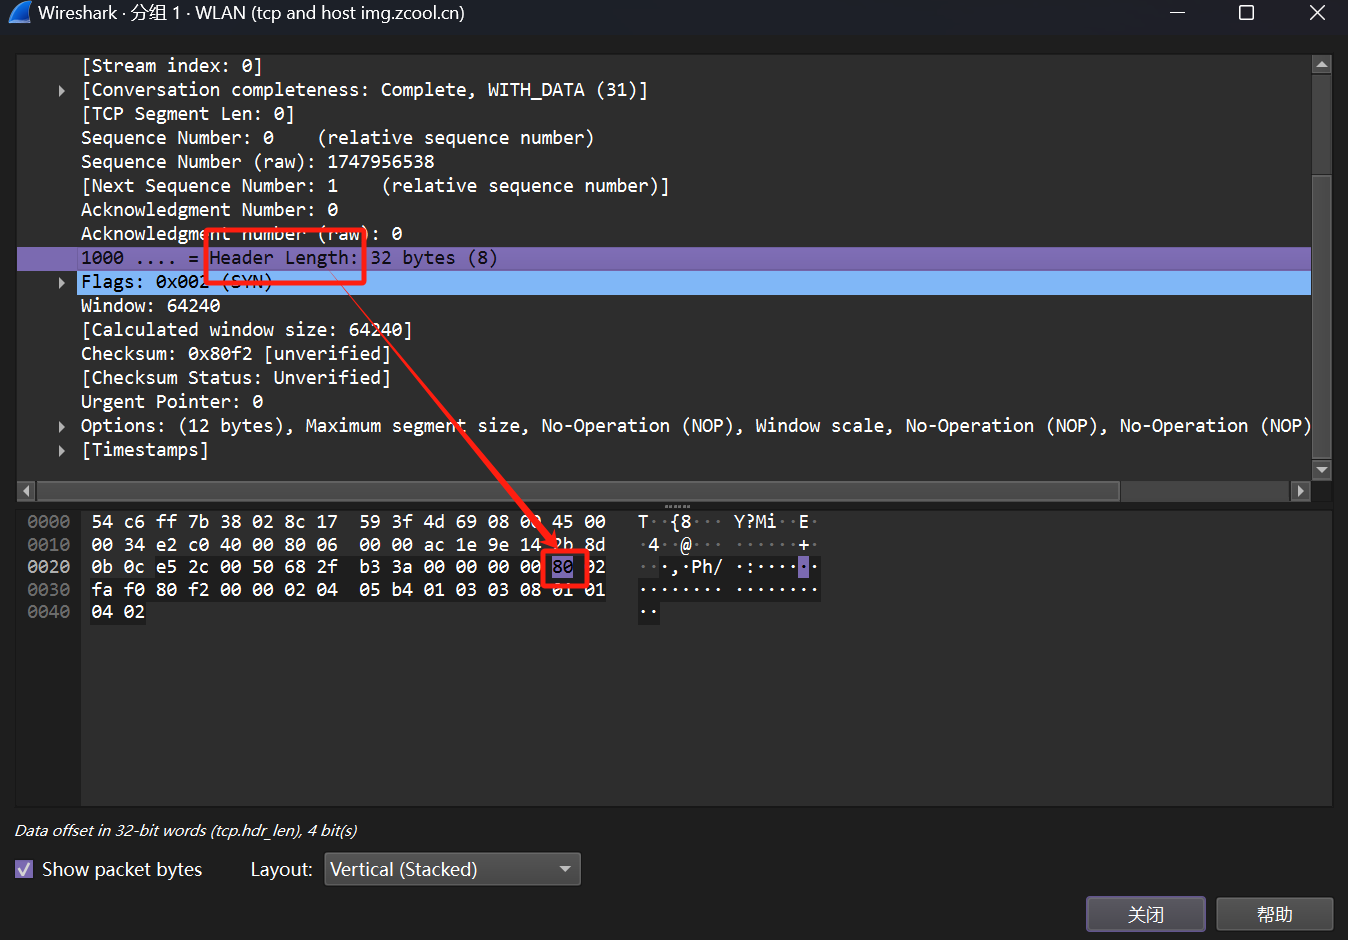
\includegraphics[width=\textwidth]{images/9.Header Length.png}
			\caption{Header Length}
		\end{minipage}
		\hfill
		\begin{minipage}[b]{0.45\textwidth}
			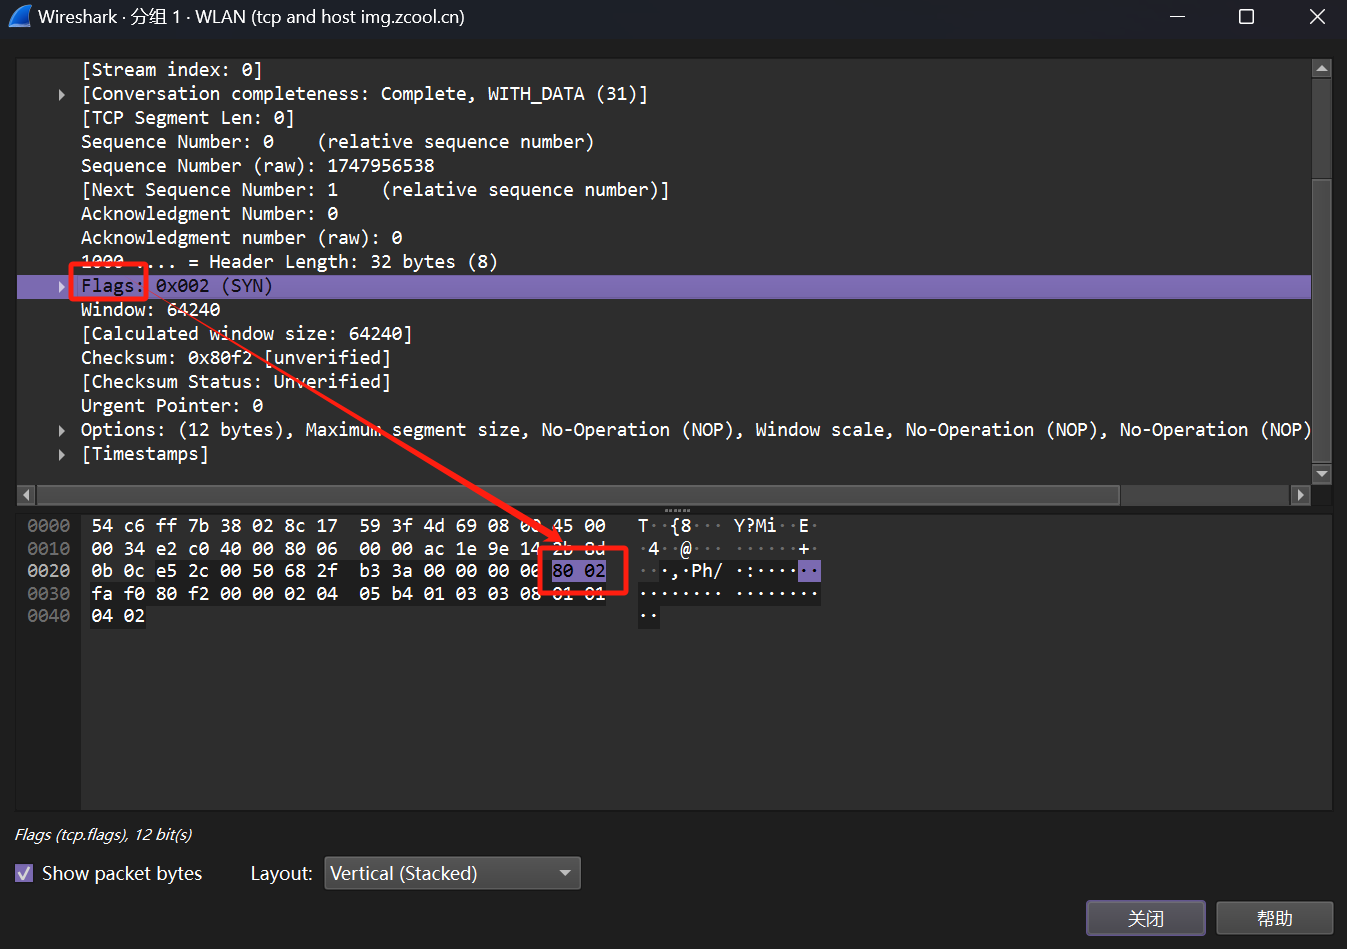
\includegraphics[width=\textwidth]{images/10.Flags.png}
			\caption{Flags}
		\end{minipage}
	\end{figure}
	
	\begin{figure}[H]
		\centering
		\begin{minipage}[b]{0.45\textwidth}
			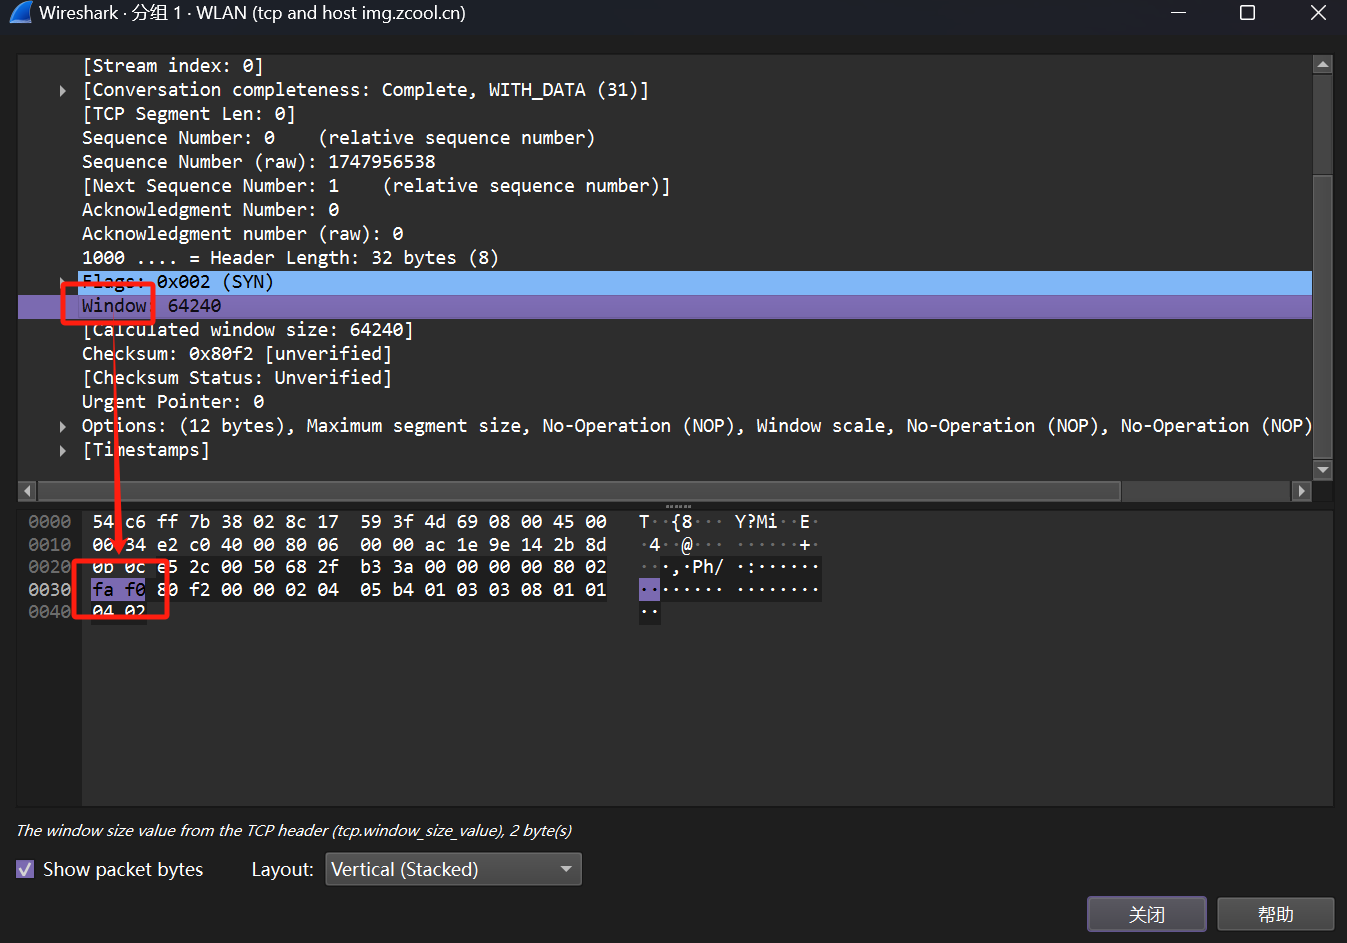
\includegraphics[width=\textwidth]{images/11.Window.png}
			\caption{window}
		\end{minipage}
		\hfill
		\begin{minipage}[b]{0.45\textwidth}
			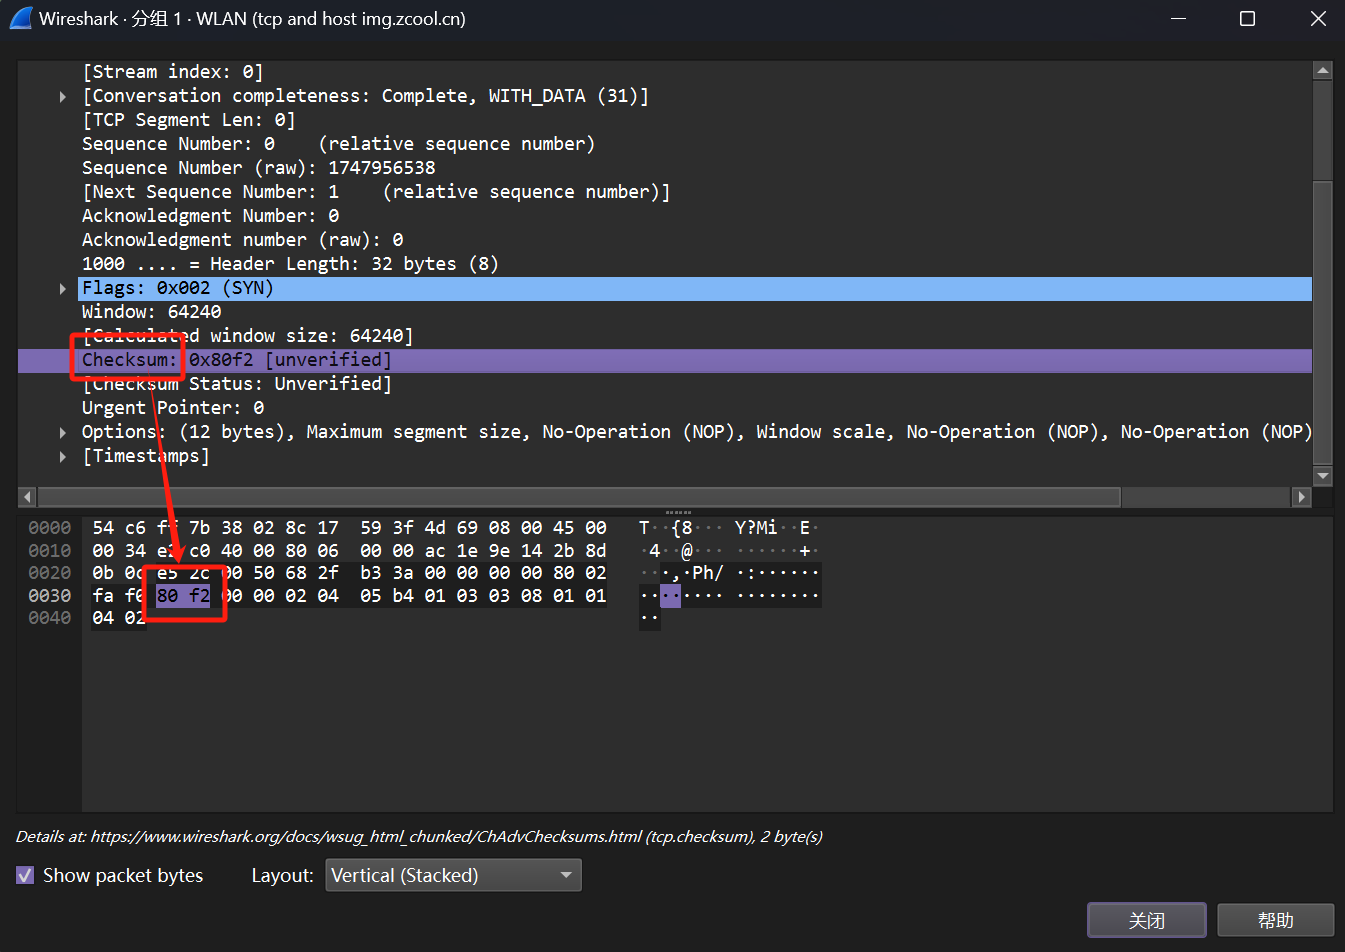
\includegraphics[width=\textwidth]{images/12.Checksum.png}
			\caption{Checksum}
		\end{minipage}
	\end{figure}
	
	\begin{figure}[H]
		\centering
		\begin{minipage}[b]{0.45\textwidth}
			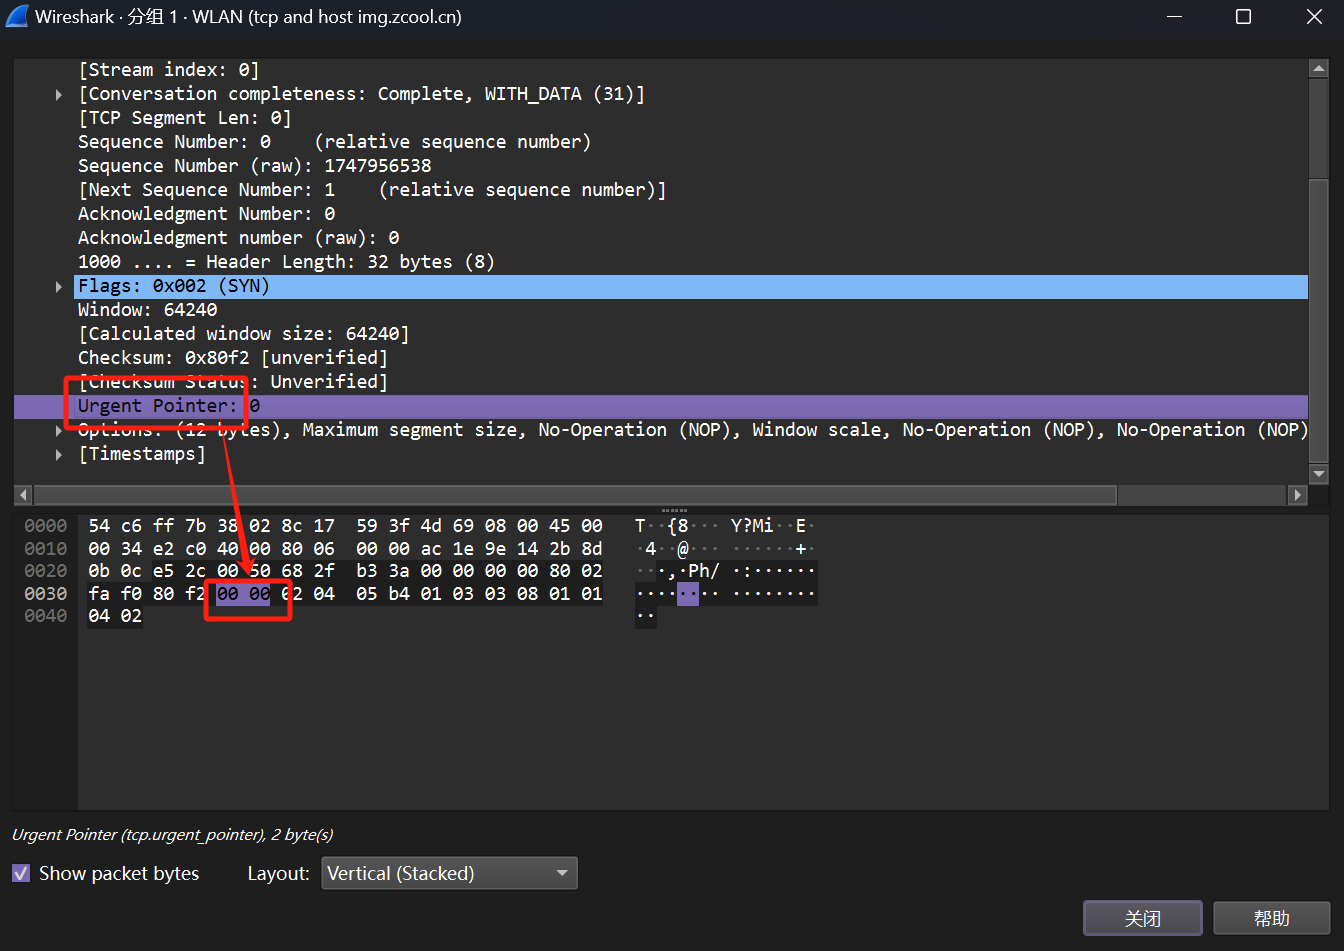
\includegraphics[width=\textwidth]{images/13.Urgent Number.png}
			\caption{Urgent Number}
		\end{minipage}
		\hfill
		\begin{minipage}[b]{0.45\textwidth}
			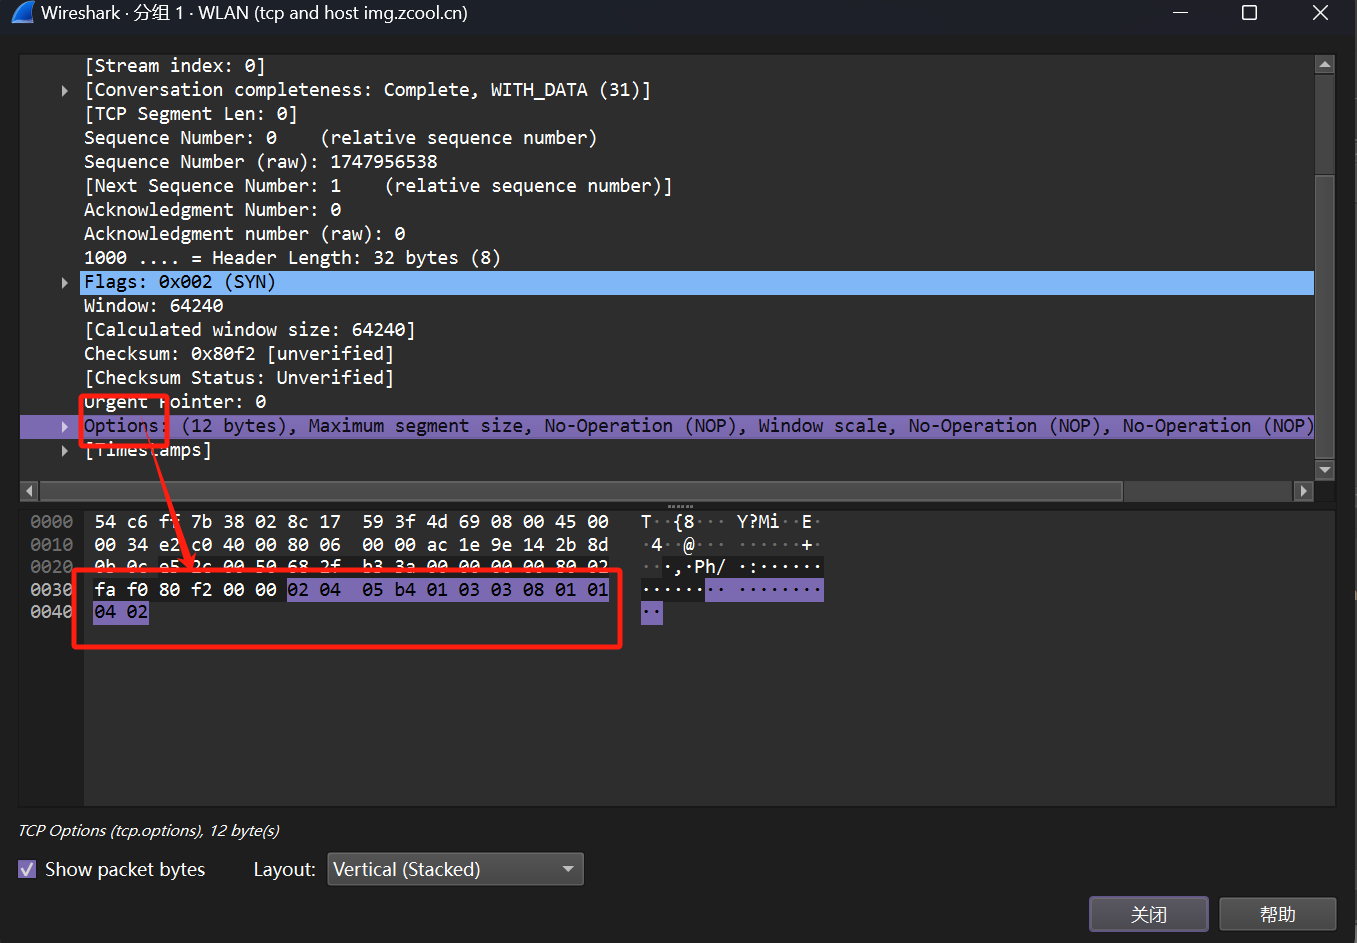
\includegraphics[width=\textwidth]{images/14.Options.png}
			\caption{Options}
		\end{minipage}
	\end{figure}
	
	可以画出\texttt{TCP}包的结构如下:
	
	\begin{figure}[H]
		\centering
		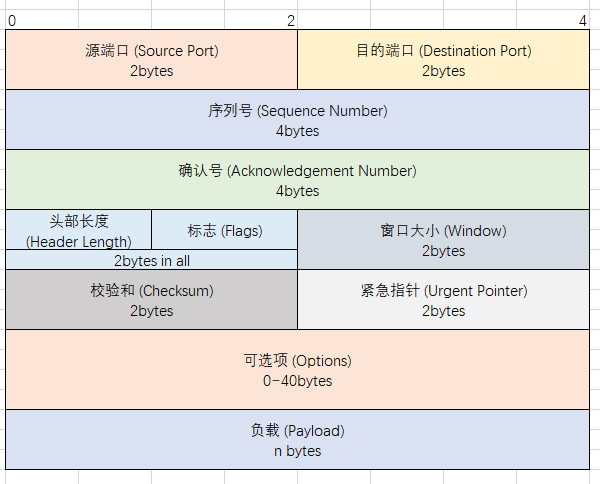
\includegraphics[width=11cm]{images/15.TCP包结构.png}
		\caption{TCP包结构}
	\end{figure}
	
	其中 \texttt{Flags} 字段包括 \texttt{Reserved}, \texttt{Accurate ECN}, \texttt{Congestion Window Reduced}, \texttt{ECN-Echo}, \\ \texttt{Urgent}, \texttt{Acknowledgment}, \texttt{Push}, \texttt{Reset}, \texttt{Syn}, \texttt{Fin}。如下图所示:
	
	\begin{figure}[H]
		\centering
		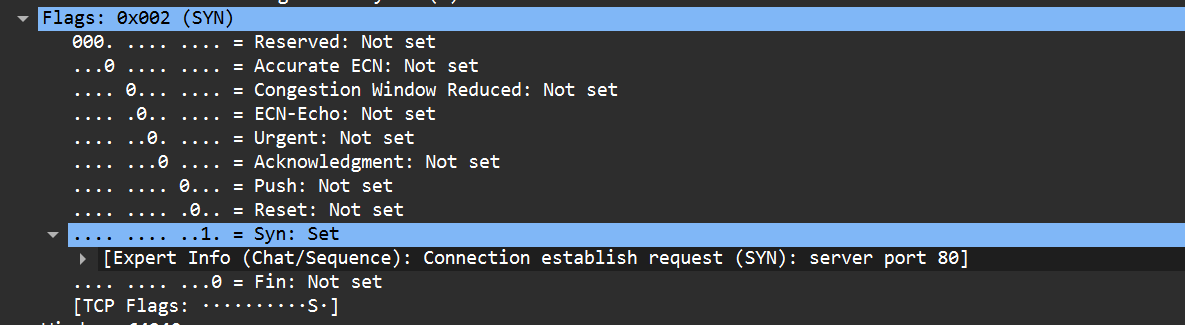
\includegraphics[width=11cm]{images/16.Flags内容.png}
		\caption{Flags}
	\end{figure}
	
	\texttt{TCP}数据包头部各字段的含义如下:
	
	\begin{itemize}[noitemsep]
		\item 源端口:源端口,占2字节,用于标识源主机的应用程序进程。
		\item 目的端口:目的端口,占2字节,用于标识目的主机的应用程序进程。
		\item 序列号:占4字节,用于标识从TCP源端向目的端发送的字节流,发送方对此进行标记。
		\item 确认号:占4字节,只有当ACK标志位为1时,确认号字段才有效,确认号等于上次接收到的字节序号加1。
		\item 头部长度:占1字节,指示TCP头部的长度。
		\item 标志:与头部长度合占2字节。各标志位的含义如下:
	
		\begin{itemize}[noitemsep]
			\item Reserved:保留位。
			\item Accurate ECN:显式拥塞通知。
			\item Congestion Window Reduced:拥塞窗口减小。
			\item ECN-Echo:显式拥塞通知回显。
			\item URG:紧急指针(urgent pointer)有效。
			\item ACK:确认号有效。
			\item PSH:接收方应尽快将此报文段交付给应用层。
			\item RST:重置连接。
			\item SYN:发起一个新连接。
			\item FIN:释放一个连接。
		\end{itemize}
		\item 窗口大小:占2字节,表示发送方在收到确认前允许发送的字节数。
		\item 校验和:占2字节,用于检验TCP首部和TCP数据的正确性。
		\item 紧急指针:占2字节,仅当URG标志为1时有效。紧急指针指出紧急数据在报文段中的位置。
		\item 可选项:占0-40字节,可选项可以有0个或多个,用于一些可选的设置。
	\end{itemize}
	
	\subsection{TCP 连接的建立和释放}
	
	\subsubsection{三次握手}
	
	\begin{enumerate}[noitemsep, label={{\arabic*})}]
		\item 第一次握手 TCP客户进程也是先创建传输控制块TCB,然后向服务器发出连接请求报文,这是报文首部中的同部位SYN=1,同时选择一个初始序列号 seq=x ,此时,TCP客户端进程进入了 SYN-SENT 同步已发送状态
		
		\item 第二次握手 TCP服务器收到请求报文后,如果同意连接,则会向客户端发出确认报文。确认报文中应该 ACK=1,SYN=1,确认号是ack=x+1,同时也要为自己初始化一个序列号 seq=y,此时,TCP服务器进程进入了 SYN-RCVD 同步收到状态
		
		\item 第三次握手 TCP客户端收到确认后,还要向服务器给出确认。确认报文的ACK=1,ack=y+1,自己的序列号seq=x+1,此时,TCP连接建立,客户端进入ESTABLISHED已建立连接状态 触发三次握手
	\end{enumerate}\textbf{}
	
	在Wireshark中,我们来观察三次握手,可以看到三次握手的过程如下:
	
	\begin{figure}[H]
		\centering
		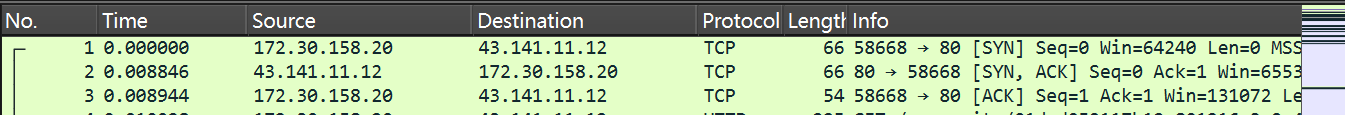
\includegraphics[width=11cm]{images/17.三次握手.png}
		\caption{三次握手}
	\end{figure}
	
	画出三次握手协议的步骤图如下:
	
	\begin{figure}[H]
		\centering
		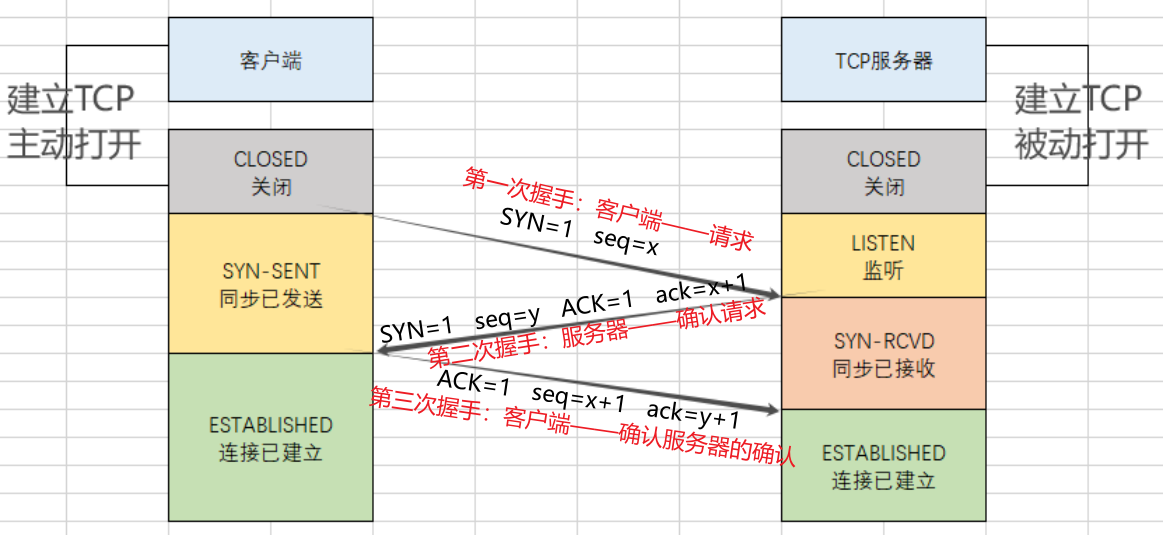
\includegraphics[width=11cm]{images/18.三次握手过程.png}
		\caption{三次握手过程}
	\end{figure}
	
	观察SYN package,如下图所示:
	
	\begin{figure}[H]
		\centering
		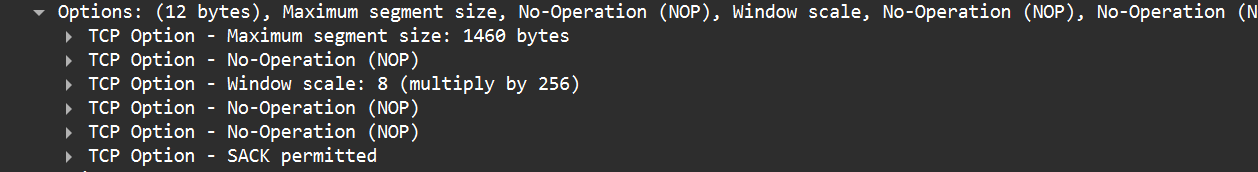
\includegraphics[width=11cm]{images/19.TCP SYN Options.png}
		\caption{TCP SYN Options}
	\end{figure}
	
	\begin{tcolorbox}[title = {Question}, colback = red!25!white, colframe = red!75!black]
		What TCP Options are carried on the SYN packets for your trace?
	\end{tcolorbox}
	
	\begin{tcolorbox}[title = {Answer}, colback = blue!25!white, colframe = blue!75!black]
		\begin{enumerate}[noitemsep, label={{\arabic*})}]
			\item \textbf{Maximum segment size}:指定最大段的大小
			\item \textbf{No-Operation}:无操作(可用于填充字节)
			\item \textbf{Window scale}:指定了窗口大小的倍数,用于调整窗口大小的限制
			\item \textbf{SACK permitted}:允许使用SACK选择确认(选择性确认)
		\end{enumerate}\textbf{}
		
		此外,还可以观察到一些其他的信息,如SYN包中包含的End of Option List、Timestamp(记录时间信息)等选项。在这个包中,Wireshark将时间戳放置在Options之外,并用中括号标记,查看时可以关注first frame和previous frame,均为0。
		
	\end{tcolorbox}
	
	\subsubsection{四次挥手}
	
	TCP的四次挥手过程如下:
	
	\begin{enumerate}[noitemsep]
		\item 客户端发送关闭连接的报文段,设置FIN标志为1,表示请求关闭连接,并停止发送数据。序列号设为 $ seq = x $(为之前发送的所有数据的最后一个字节序号加1),客户端进入FIN-WAIT-1状态,等待服务器的确认报文。
		\item 服务器收到FIN报文后,发送确认报文,设置ACK为1,且ack $ = x + 1 $,带上自己的序列号 $ seq = y $。此后,服务器进入CLOSE-WAIT状态,并通知上层应用程序该连接已释放,但仍然可以接收数据。
		\item 客户端收到服务器的ACK报文后,进入FIN-WAIT-2状态,此时仍能够接收来自服务器的数据。
		\item 服务器在发送完所有数据后,会发送自己的FIN报文,并等待客户端的ACK确认。此时服务器进入LAST-ACK状态。
		\item 客户端收到服务器的FIN报文后,会反馈一个ACK报文,告知服务器已接收,进入TIME-WAIT状态,等待 $ 2MSL $(2倍报文段最大存活时间)。此时网络中可能存留最长时间的报文为30秒、1分钟或2分钟。如果没有特殊情况,客户端最终会进入CLOSED状态。
		\item 服务器收到客户端的ACK报文后,进入CLOSED状态,结束连接过程。
	\end{enumerate}
	
	在Wireshark中,我们来观察四次挥手,可以看到四次挥手的过程如下:
	
	\begin{figure}[H]
		\centering
		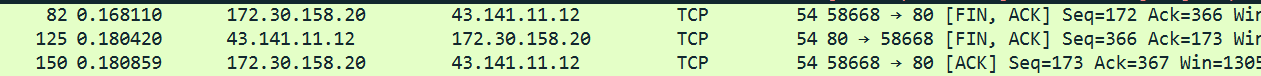
\includegraphics[width=11cm]{images/20.四次挥手.png}
		\caption{四次挥手}
	\end{figure}
	
	画出四次挥手协议的步骤图如下:
	
	\begin{figure}[H]
		\centering
		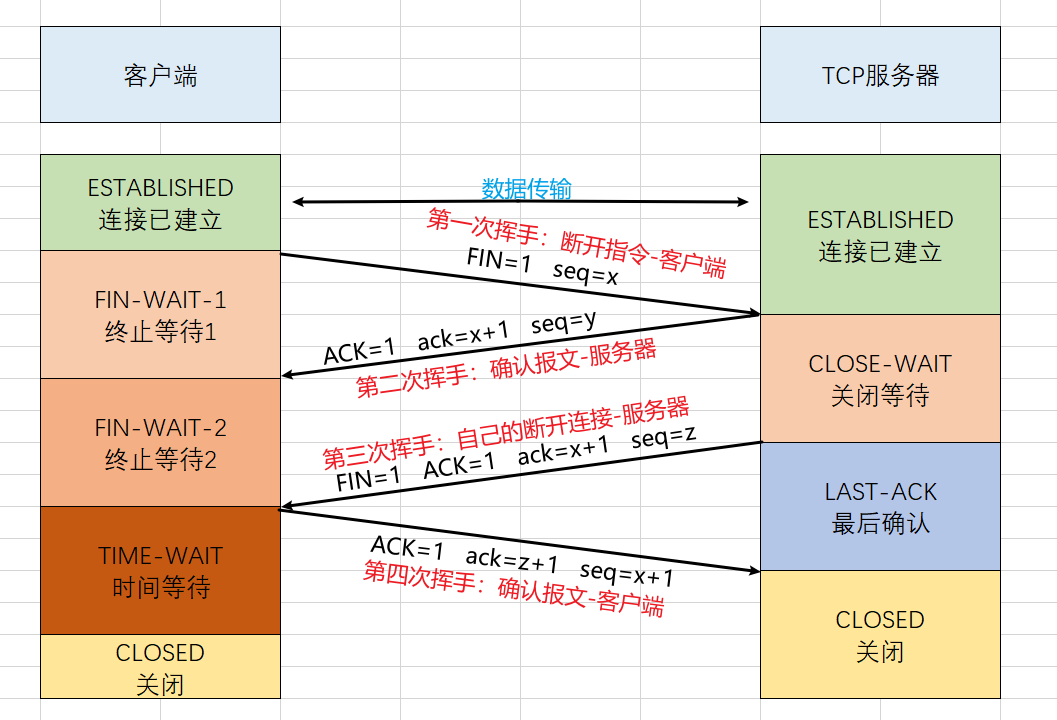
\includegraphics[width=11cm]{images/21.四次挥手过程.png}
		\caption{四次挥手过程}
	\end{figure}
	
	回答问题:
	
	\begin{tcolorbox}[title = {Question}, colback = red!25!white, colframe = red!75!black]
		为什么建立连接时使用三次握手,而释放连接时四次挥手?
	\end{tcolorbox}
	
	\begin{tcolorbox}[title = {Answer}, colback = blue!25!white, colframe = blue!75!black]
		当一方接收到另一方发送的\texttt{FIN}包时,可能还有一些数据包尚未发送。因此,它会首先回复一个\texttt{ACK}包,待所有的数据包处理完毕并发送完后,随后再发送\texttt{FIN ACK}包以确认关闭连接。在此过程中,对方收到\texttt{FIN ACK}包后,会再回复一个\texttt{ACK}包。而在连接的建立过程中不会出现这样的情况,因此只需三次握手便可完成连接的建立。
	\end{tcolorbox}
	
	\subsection{TCP 数据传输}
	
	在Static统计菜单下,选择“IO”图表,以查看数据包的传输速率。
	
	为了方便观察,将间隔改为100ms,Y轴改为Bits,
	
	\begin{enumerate}[noitemsep, label={{\arabic*})}]
		\item 调整过滤器为“tcp.srcport==80”,只查看下载数据包,重新绘图
		\item 调整过滤器为“tcp.dstport==80”,只查看上传数据包,重新绘图
	\end{enumerate}\textbf{}
	
	观察 \texttt{Wireshark} 生成的 \texttt{IO} 图表, 如下所示:
	
	\begin{figure}[H]
		\centering
		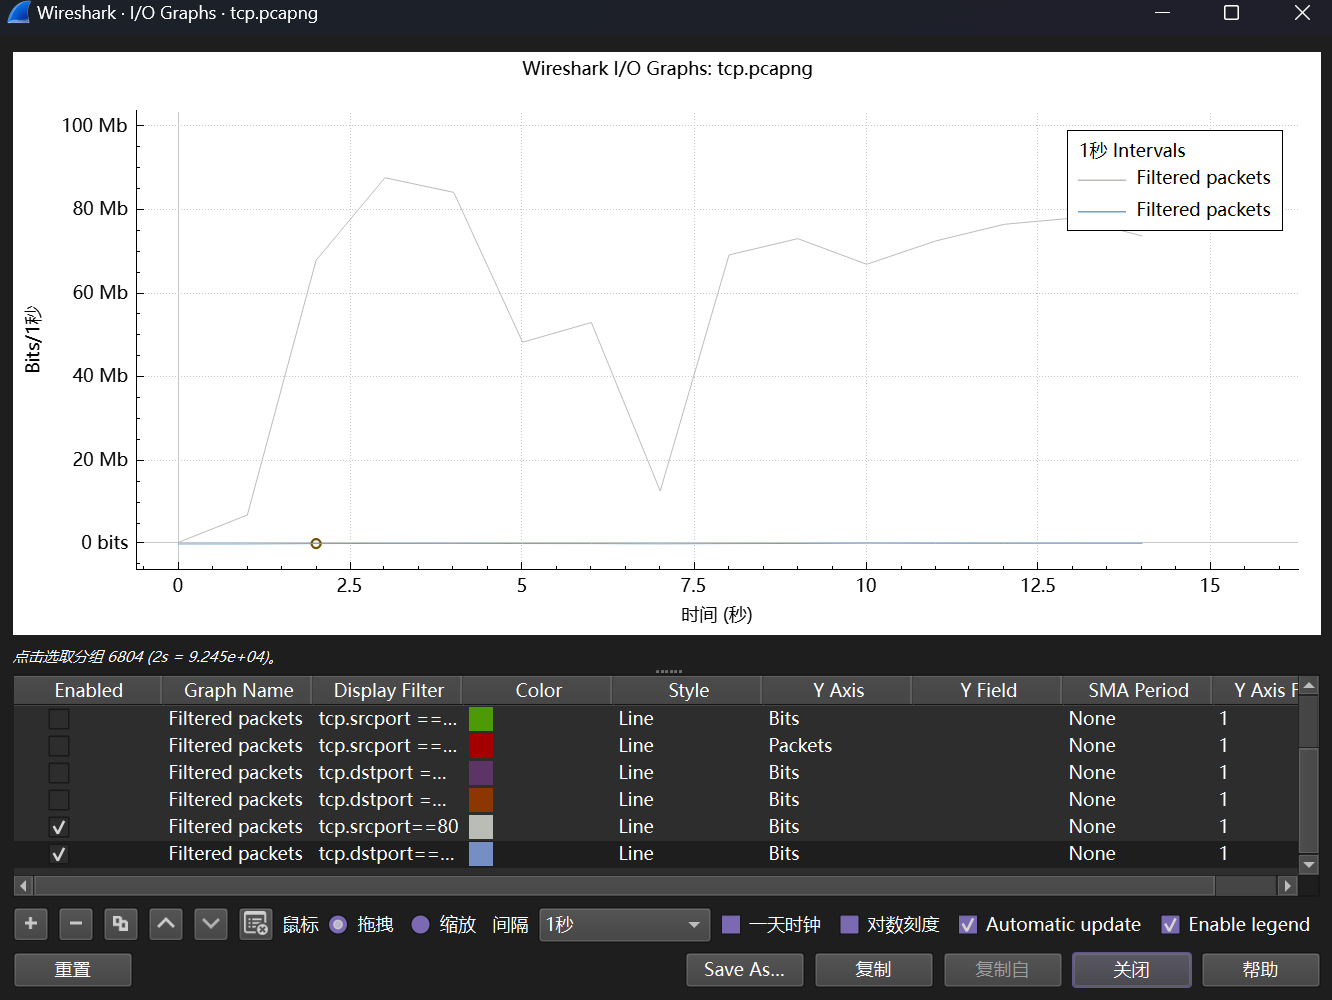
\includegraphics[width=11cm]{images/22.TCP Data Transfer.png}
		\caption{TCP Data Transfer}
	\end{figure}
	
	\begin{tcolorbox}[title = {Question-1}, colback = red!25!white, colframe = red!75!black]
		What is the rough data rate in the download direction in packets/second and bits/second once the TCP connection is
		running well?
	\end{tcolorbox}
	
	\begin{tcolorbox}[title = {Answer-1}, colback = blue!25!white, colframe = blue!75!black]
		根据表格可以看出,下载速率到达3000kb+/100ms,也就是$ 3*10^8 bits/s $,下载速率到达大约$ 1.8*10^8 bits/s $
	\end{tcolorbox}
	
	\begin{tcolorbox}[title = {Question-2}, colback = red!25!white, colframe = red!75!black]
		What percentage of this download rate is content? Show your calculation. To find out, look at a typical download packet; there should be many similar, large download packets. You can see how long it is, and how many bytes of TCP payload it contains.
	\end{tcolorbox}
	
	\begin{tcolorbox}[title = {Answer-2}, colback = blue!25!white, colframe = blue!75!black]
		选中一个数据包观察:
		
		\begin{figure}[H]
			\centering
			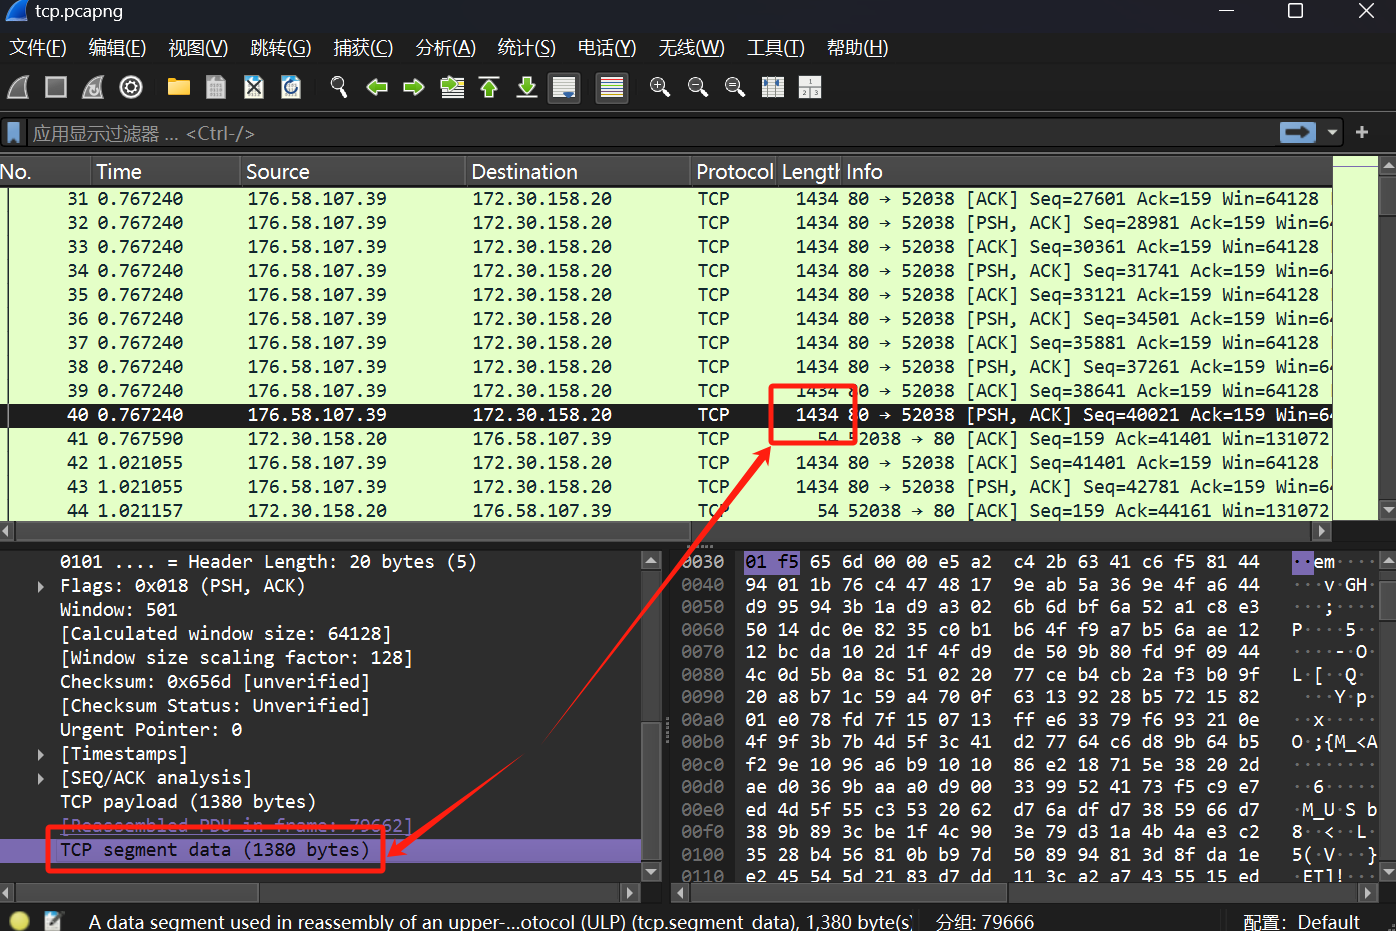
\includegraphics[width=11cm]{images/23.TCP Packet.png}
			\caption{TCP Packet}
		\end{figure}
		
		可以看到其总大小为1434字节,其中 TCP 负载部分为 1380 字节,占比约为96.23\%.
	\end{tcolorbox}
	
	\begin{tcolorbox}[title = {Question-3}, colback = red!25!white, colframe = red!75!black]
		What is the rough data rate in the upload direction in packets/second and bits/second due to the ACK packets?
	\end{tcolorbox}
	
	\begin{tcolorbox}[title = {Answer-3}, colback = blue!25!white, colframe = blue!75!black]
		观察可得,平均值约为 $ 1.0 × 10^5 $ Bits/s, 最大值达到了$ 2.0 × 10^5 $ Bits/s 。
		
		\begin{figure}[H]
			\centering
			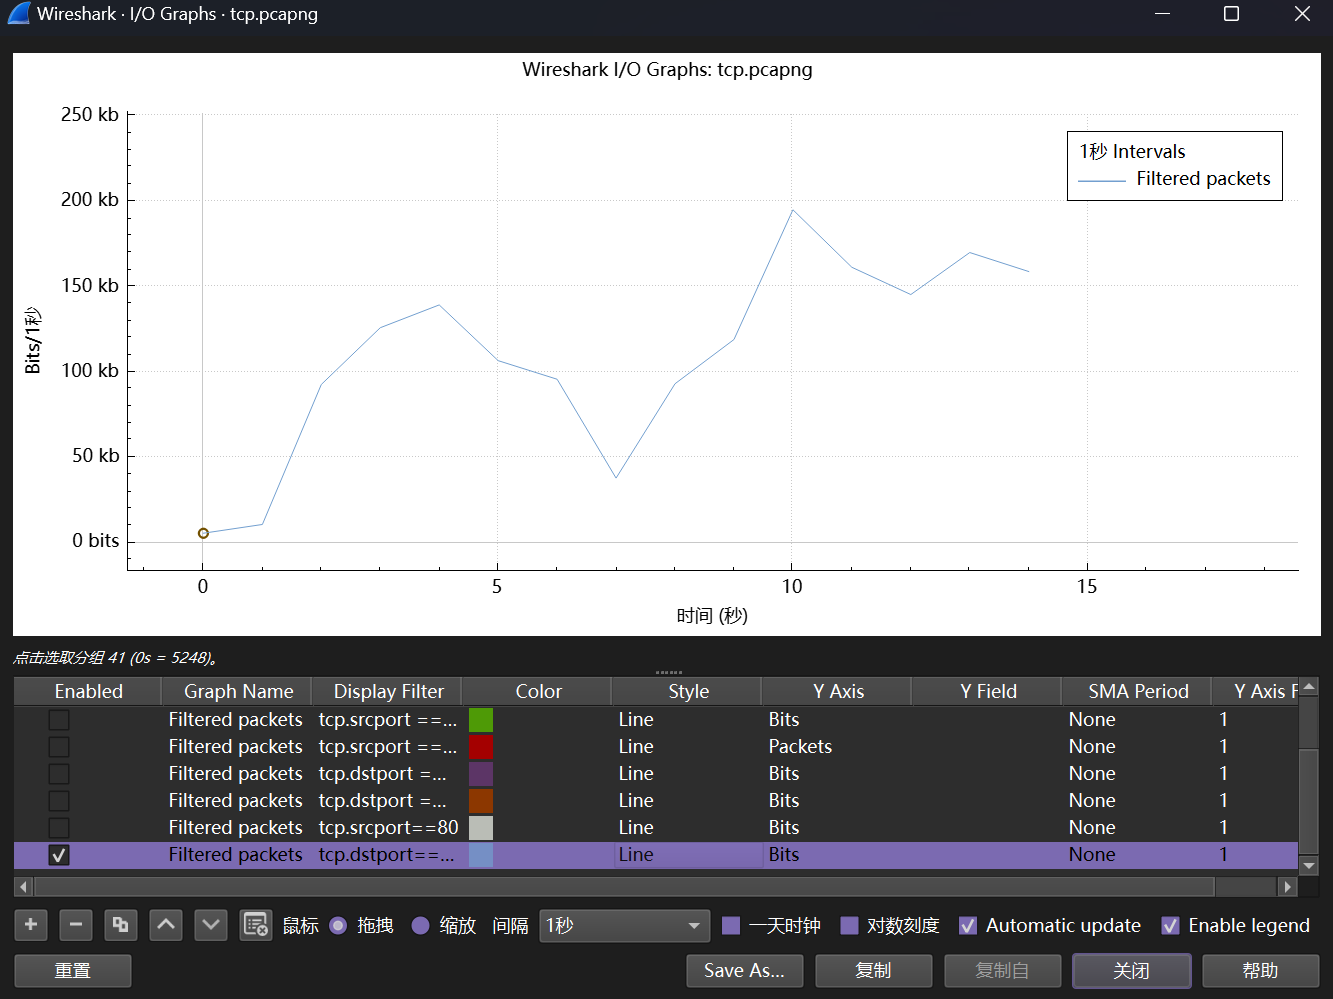
\includegraphics[width=11cm]{images/24.ACK Rough data rate.png}
			\caption{ACK Rough data rate}
		\end{figure}
	\end{tcolorbox}
	
	\begin{tcolorbox}[title = {Question-4}, colback = red!25!white, colframe = red!75!black]
		If the most recently received TCP segment from the server has a sequence number of X, then what ACK number does the next transmitted TCP segment carry?
	\end{tcolorbox}
	
	\begin{tcolorbox}[title = {Answer-4}, colback = blue!25!white, colframe = blue!75!black]
		Ack告诉下一个期望的序列号,因此下一个发送的ACK 是X + Segment Len
	\end{tcolorbox}
	
	\subsection{问题讨论}
	
	因为想要更好的展现数据,所以这里通过以下命令,选择一个100MB的照片来下载,重新wget:
	
	\begin{lstlisting}[language=bash]
    C:\User\GHOST> wget http://speedtest.london.linode.com/100MB-london.bin
	\end{lstlisting}
	
	\begin{figure}[H]
		\centering
		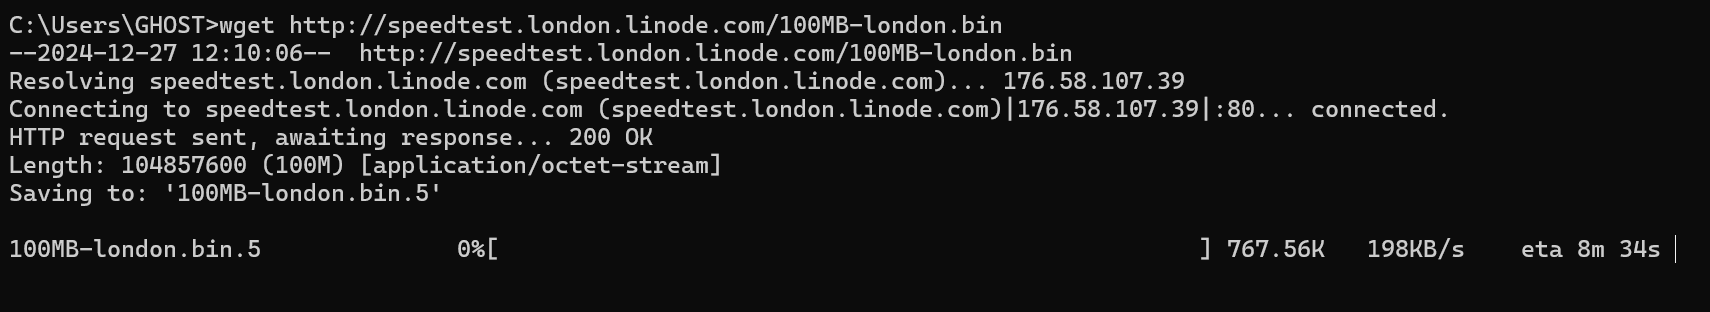
\includegraphics[width=9cm]{images/25.Get 100MB File.png}
		\caption{Get 100MB File}
	\end{figure}
	
	\begin{figure}[H]
		\centering
		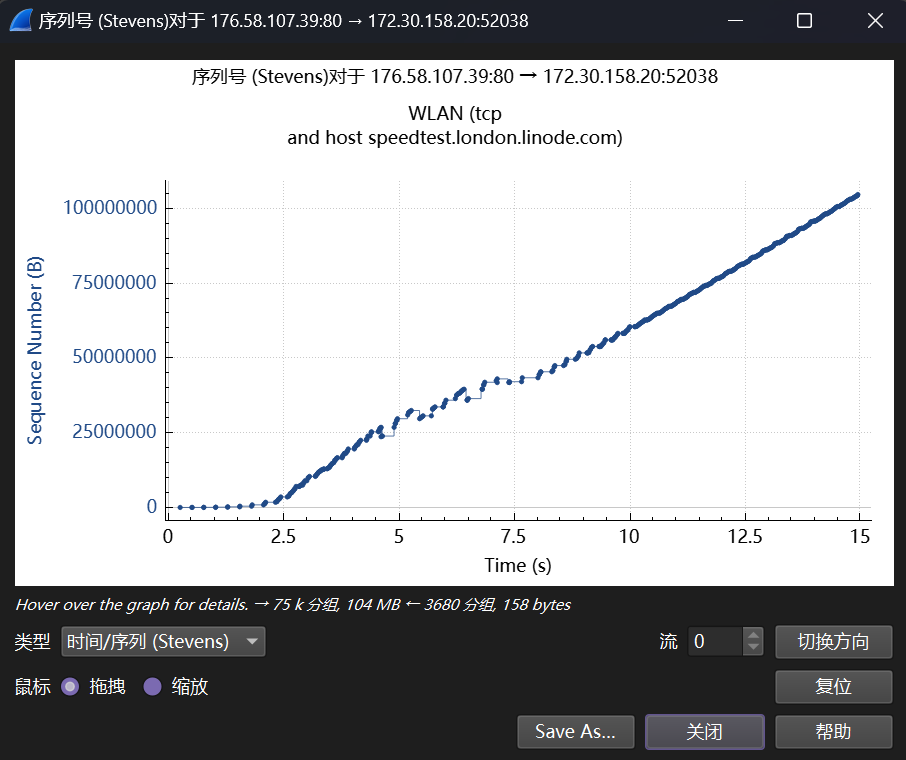
\includegraphics[width=11cm]{images/26.序列号.png}
		\caption{序列号}
	\end{figure}
	
	\begin{figure}[H]
		\centering
		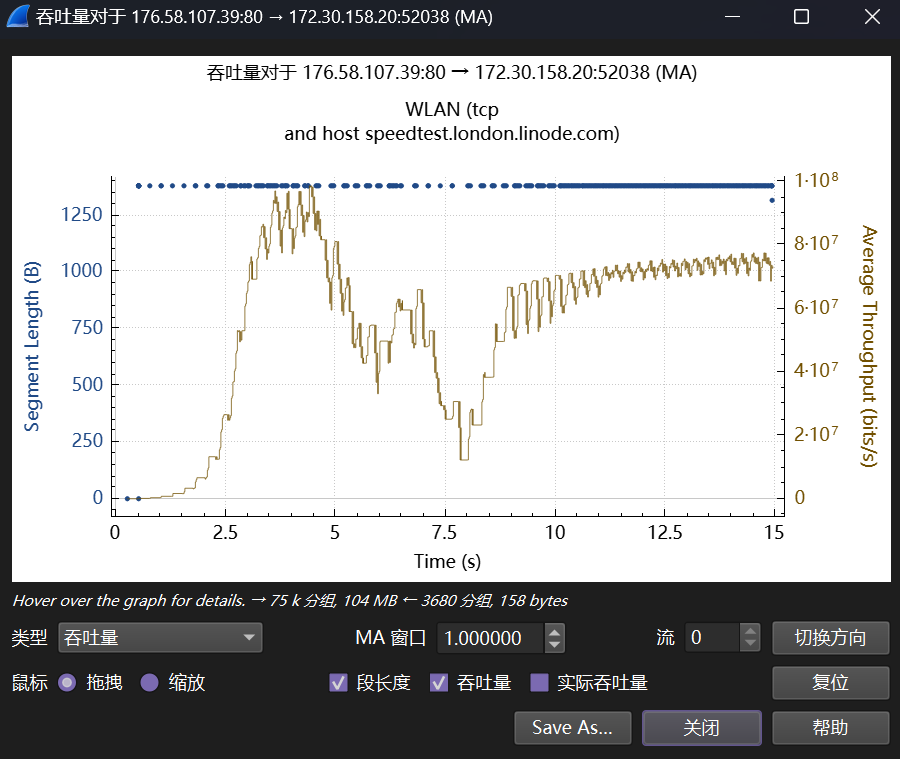
\includegraphics[width=11cm]{images/27.吞吐量.png}
		\caption{吞吐量}
	\end{figure}
	
	\begin{figure}[H]
	\centering
	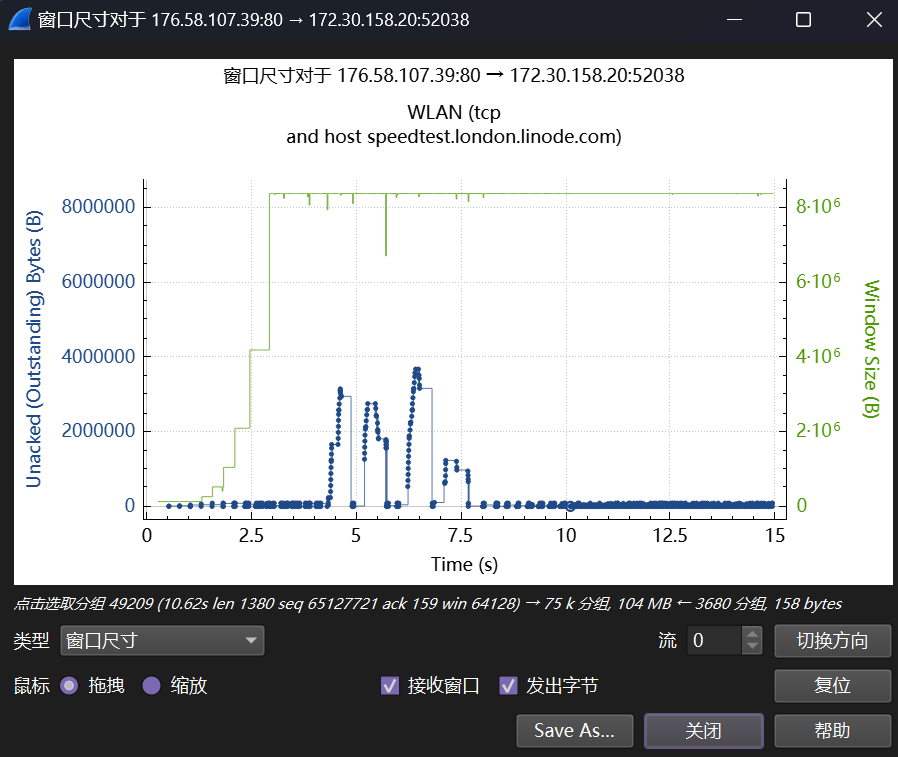
\includegraphics[width=11cm]{images/28.窗口尺寸.png}
	\caption{窗口尺寸}
	\end{figure}
	
	\begin{figure}[H]
	\centering
	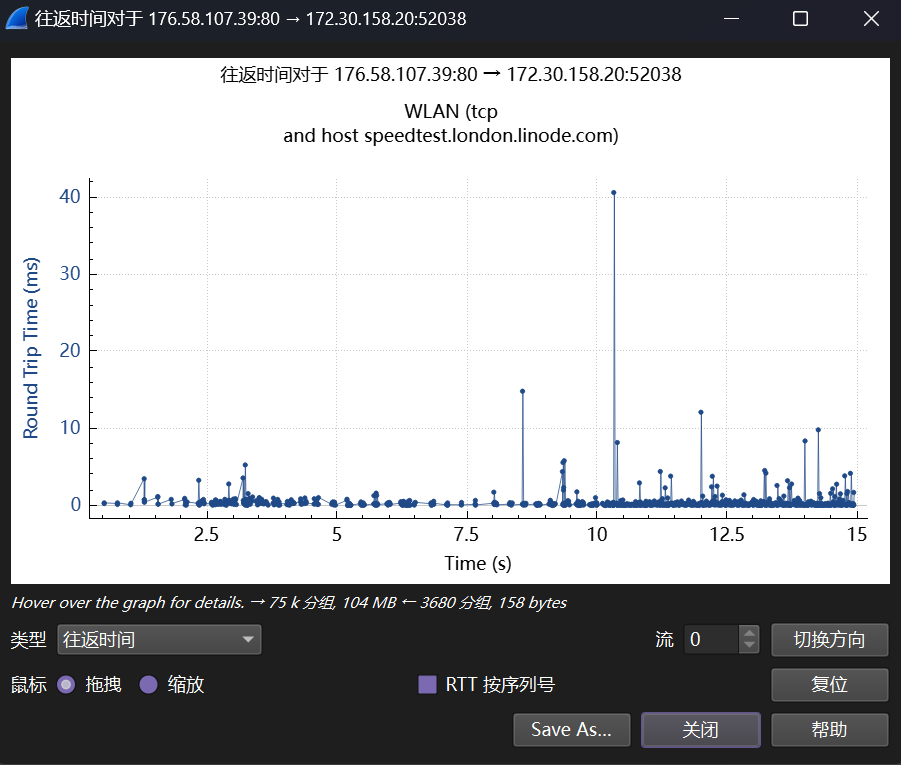
\includegraphics[width=11cm]{images/29.往返时间.png}
	\caption{往返时间}
	\end{figure}
	
	回答以下问题:
	
	\begin{tcolorbox}[title = {Question-1}, colback = red!25!white, colframe = red!75!black]
		Explore the congestion control and the classic AIMD behavior of TCP.  To do this, you will likely want to capture a trace while you are sending (not receiving) a moderate amount of data on a TCP connection. You can then use the “TCP Stream Graph” tools as well as other analysis to observe how the congestion window changes over time.
	\end{tcolorbox}
	
	\begin{tcolorbox}[title = {Answer-1}, colback = blue!25!white, colframe = blue!75!black]
		从吞吐量表中可以观察到,吞吐量随着时间的推移而上升,但在特定时间点会经历急剧下降并出现波动。这种波动是由于网络拥堵事件导致的,此时传输控制协议(TCP)会调整其拥塞窗口大小,随后逐渐恢复,这一动态调整过程即为拥塞管理机制。
	\end{tcolorbox}
	
	\begin{tcolorbox}[title = {Question-2}, colback = red!25!white, colframe = red!75!black]
		Explore the reliability mechanisms of TCP more deeply. Capture a trace of a connection that includes segment loss. See what triggers the retransmissions and when. Also look at the round-trip time estimator.
	\end{tcolorbox}
	
	\begin{tcolorbox}[title = {Answer-2}, colback = blue!25!white, colframe = blue!75!black]
		当检测到数据包未能按预期顺序到达时(这通常是由于早期的数据包在传输过程中丢失),将激活数据重传流程,以确保丢失的数据包得到补充。**往返时间图表已在上方列出
		
		\begin{figure}[H]
			\centering
			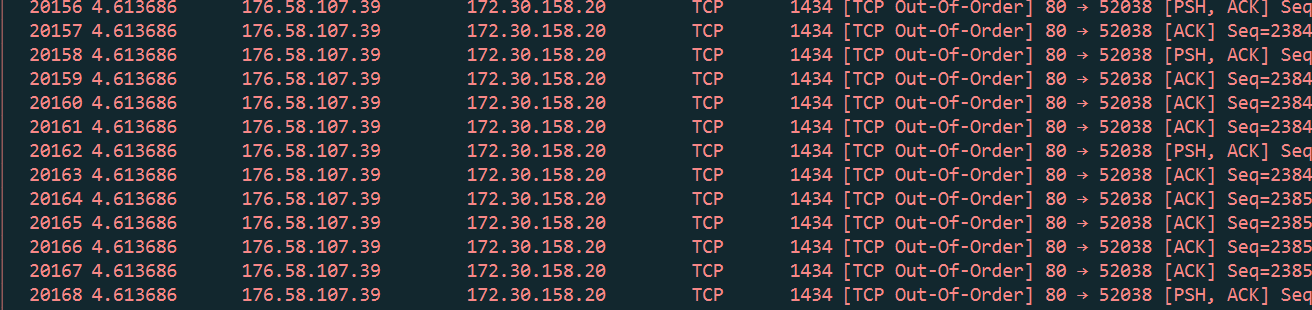
\includegraphics[width=11cm]{images/30.错误重传.png}
			\caption{错误重传}
		\end{figure}
	\end{tcolorbox}
	
	\begin{tcolorbox}[title = {Question-3}, colback = red!25!white, colframe = red!75!black]
		Look at the use of options including SACK to work through the details. You should see information about ranges of received bytes during times of segment loss.
	\end{tcolorbox}
	
	\begin{tcolorbox}[title = {Answer-3}, colback = blue!25!white, colframe = blue!75!black]	
		观察一个Options中包含SACK的数据包,如下图所示:
		
		\begin{figure}[H]
			\centering
			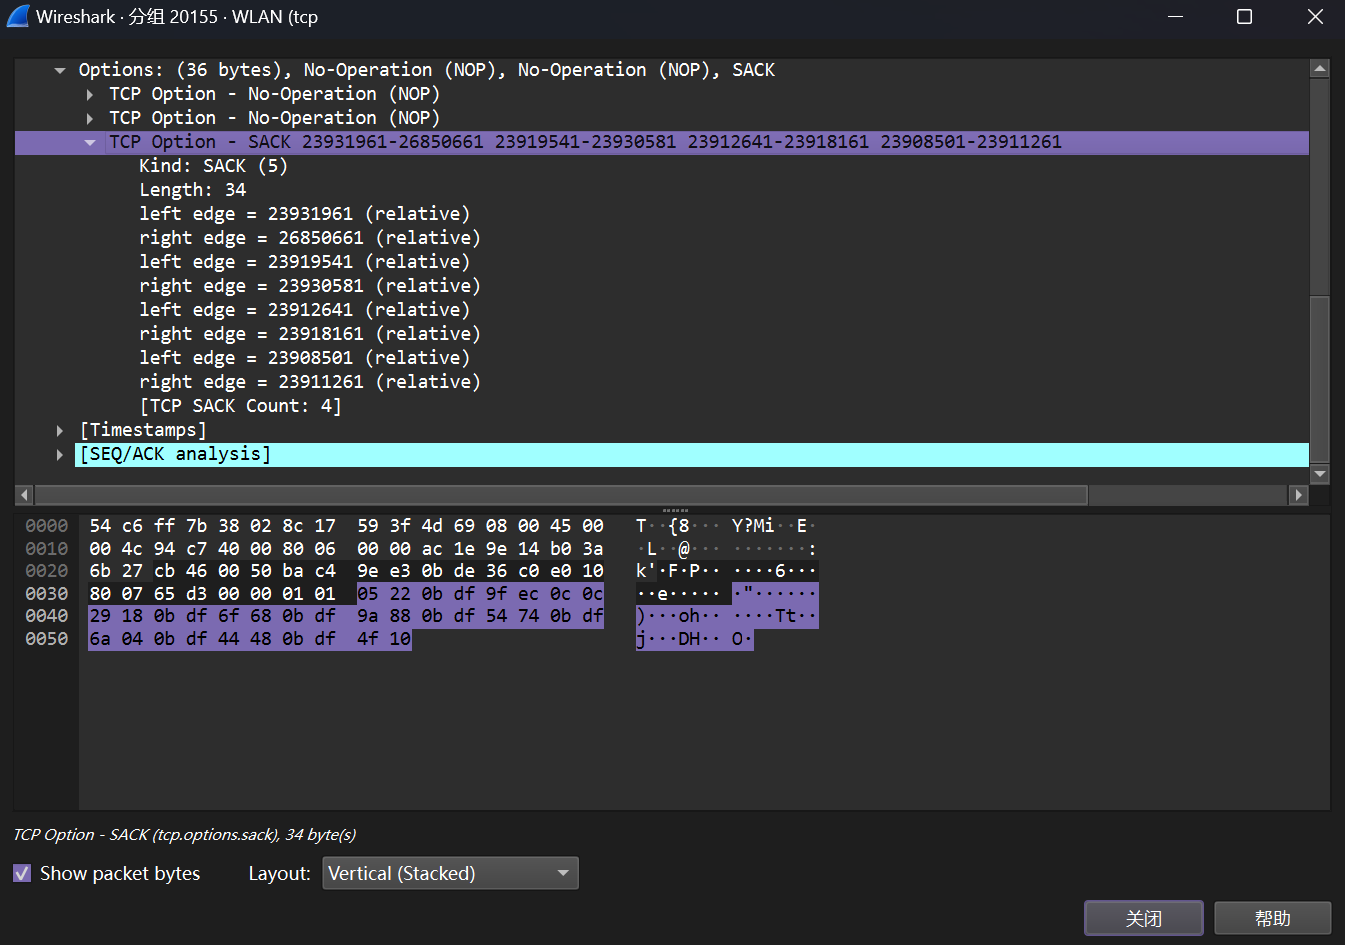
\includegraphics[width=11cm]{images/31.SACK.png}
			\caption{SACK}
		\end{figure}
		
		可以看到,SACK 中包含了丢失的数据包的序列号范围。
	\end{tcolorbox}
	
	\begin{tcolorbox}[title = {Question-4}, colback = red!25!white, colframe = red!75!black]
		TCP is the transport layer underlying the web. You can see how your browser makes use of TCP by setting up concurrent connections.
	\end{tcolorbox}
	
	\begin{tcolorbox}[title = {Answer-4}, colback = blue!25!white, colframe = blue!75!black]
		在处理用户发起的网络请求时,浏览器通常会创建多个TCP连接,以便并行处理这些请求。
	\end{tcolorbox}
	
	\section{实验结果总结}
	
	在本实验环节,我深入探究了传输控制协议(TCP)的数据包构成,并掌握了其连接的建立与终止流程,同时对数据传输机制有了全面的认识。
	
	此外,我还对TCP的流量控制原理和确保数据传输可靠性的方法进行了学习。
	
	\section{附录}
	
	无
	
\end{document}
